\documentclass[a4paper,11pt]{article}
\usepackage{graphicx} % Required for inserting images
\usepackage[english]{babel}
\usepackage[latin1]{inputenc}
\usepackage[top=2cm,bottom=2cm, left=2cm, right=2cm]{geometry}
\usepackage{subcaption}
\usepackage{hyperref}
\usepackage{siunitx}
\setlength{\parindent}{0pt}
\usepackage{parskip}
\usepackage{booktabs}
\usepackage{subfiles}
\usepackage[numbers]{natbib}
\usepackage{amsmath}
\usepackage{float}

%figures and subfigures
\usepackage{caption}
\usepackage{subcaption}

\usepackage{setspace}
\onehalfspacing

\usepackage[toc,page]{appendix} %allows fancyhdr and notoccite together
\usepackage{notoccite} %references in captions numbering

\usepackage{fancyhdr}
\fancypagestyle{main}{%
  \fancyhf{}
  \fancyhead[L]{\nouppercase{\leftmark}}%
  \fancyhead[R]{Page \thepage}%
  \renewcommand{\headrulewidth}{0.5pt}%
  \setlength{\headheight}{14pt}
  \setlength{\headsep}{15pt}
  \addtolength{\topmargin}{15pt}
}

\sisetup{per-mode = symbol}




\title{FYP}
\author{Luca Mazzotta}
\date{May 2023}


\begin{document}



\pagestyle{plain}
\pagenumbering{roman}

\begin{titlepage}
\vspace*{-2cm}
\centerline{\makebox[\textwidth]{
\includegraphics[width=\paperwidth]{Images/cover_page_header.png}}}
\vspace{2cm}

\centering

\vspace{-2cm}

\newcommand{\HRule}{\rule{\linewidth}{0.5mm}} % Defines a new command for the horizontal lines, change thickness here
 
\center % Center everything on the page
 
% \setlength{\topmargin}{0in}
 
 
% \textsc{\Large Final year project}\\[0.5cm] % Major heading such as course name
 
%----------------------------------------------------------------------------------------
%             TITLE SECTION
%----------------------------------------------------------------------------------------
 
\HRule \\[0.4cm]
{ \huge \bfseries Hypersonic foldable Aeroshell for THermal protection using ORigami (HATHOR) Aerothermal analysis}\\[0.4cm] % Title of your document
{\large Final Year Project}
\HRule \\[3cm]
 
\title{\line(1,0){250}\\ADM02: Mission Design and Analysis\\\line(1,0){250}}
\vspace{-2.5cm} 

%----------------------------------------------------------------------------------------
%             AUTHOR SECTION
%----------------------------------------------------------------------------------------
\vspace{0.5cm}
\begin{tabular}{rl}
\centering
{\bf Student:} & Luca Mazzotta
\\
{\bf CID:} & 01782839
\\
{\bf    Date:} & {05/06/2023}
\\
\\
{\bf Supervisor:} & Dr. Paul Bruce
\\
{\bf Second marker:} & Dr. Maria Ribera Vicent
\\
\\
{\bf Department:} & {Department of Aeronautics}  
\\
{\bf    Course:} & {H415 MEng Aeronautics}
\\
{} & {with Spacecraft Engineering}  


\\
{\bf    Academic year:} & {2022/2023}     


  
\end{tabular}

\begin{center}

{Department of Aeronautics\\
South Kensington Campus\\
Imperial College London\\
London SW7 2AZ\\
U.K.\\}
\end{center}

\vspace{0.5cm}

\vfill % Fill the rest of the page with white space

\end{titlepage}  
\newpage

\begin{abstract}
    \noindent{Given the recent increase in interest in space exploration and the relevance of rarefied hypersonics in the development of the next generation entry vehicles, a research into the effects of global and local Knudsen number on heat transfer was deemed worth to pursue. The theoretical background for rarefied flow was outlined, and relevant research in the field was examined. It was concluded that the optimal simulation method to carry out said research was Direct Simulation Monte Carlo. The method was thus explored, and four sets of simulations were designed: varying global Knudsen number, varying edge radius, varying angle of attack and constant local Knudsen number. The simulation were designed around simple geometries, such as circles and squares, in order to limit the number of variables. Convergence studies were thus carried out and the simulation results validated. From the simulations a drastic change in flow physics with rarefaction was noted, and a theoretical explanation was provided. Moreover, the dependence of the ratio between the peak and stagnation Stanton numbers on a cube with Knudsen number were investigated. No conclusive evidence was however found, and the need for further studies was pointed out.}
\end{abstract}
\newpage

\renewcommand{\abstractname}{Ringraziamenti}
\begin{abstract}
\noindent{Ai miei genitori e ai miei nonni, a cui desidero esprimere la mia gratitudine per l'amore e l'attenzione dedicati nel trasmettermi il valore della perseveranza e dell'impegno.}
\end{abstract}
\newpage

\tableofcontents
\newpage

\addcontentsline{toc}{section}{List of Figures}
\listoffigures
\newpage

\addcontentsline{toc}{section}{List of Tables}
\listoftables
\newpage

\pagestyle{main}
\pagenumbering{arabic}



\section{Introduction and motivation}
\label{1}
The last decade has seen a remarkable resurgence in attention towards space exploration. After several years of decay from the heights of the moon missions, the renewed interest from governmental bodies and private companies, the technological advancements in material science and reusable rockets, and the reemergence of human spaceflight have generated a positive feedback loop that has directed major investments into the sector.

Many groundbreaking endeavours have emerged: the rise of private space companies, led by industry giants such as Elon Musk's SpaceX and Jeff Bezos' Blue Origin, has democratized and made more accessible the space sector. Revolutionary new launchers, such as the fully reusable Falcon and the super heavy Starship (with the latter recently undergoing its first test flight), have axed the cost barrier for launching payload into space, opening up unprecedented opportunities for scientific research, commercial ventures, and space exploration.

Many national and international space agencies have also demonstrated a significant increase in interest. Among various mission of the European Space Agency (ESA), the following are noteworthy:

\begin{itemize}
    \item JUICE (launched on 14 April 2023): tasked with the exploration of Jupiter's icy moons (Europa, Ganymede and Callisto), housing a magnetometer made by Imperial College.
    \item ExoMars (initially scheduled for the second half of 2023, but currently postponed to 2028): ESA's astrobiology mission designated to investigate signs of past life on the red planet.
    \item Hera (scheduled to launch in October 2024): a mission towards the Didymos binary asteroid system tasked with examining the aftermath of a the collision between the aforementioned asteroid and DART (a previous NASA mission which investigated a method of planetary defense against near-Earth objects).
\end{itemize}

On the other side of the ocean, NASA has been engaged with building and launching the Webb space telescope.  Currently stationed at the sun-earth L2 Lagrange point, it is expected to make groundbreaking discoveries thanks to its infrared camera, which will allow to see objects too distant or faint to be captured by earth-stationed telescopes or the Hubble telescope.

Meanwhile, NASA's Artemis program (in collaboration with ESA and JAXA) plans to establish a long-term human presence on the moon, through the construction of a permanent outpost on the lunar surface. An extraterrestrial space station, called Gateway, will also be built. It will be placed into lunar orbit and will serve as a communication hub and temporary habitation module for astronauts in deep space missions.

The increased interest in space exploration has led to the need to efficiently launch and land greater and greater payloads has emerged. While progress on the former objective has been very good (thanks, for example, to reusable rockets such as the aforementioned Falcon and Starship, or the more conventional Space Launch System), advancements in the latter area are still lacking.

\subsection{Entry, descent and landing}
Getting a spacecraft to safely land onto the surface of a planet is a complex undertaking, characterised by significant challenges \cite{aerothermonotes}. It is composed by three parts: 
\begin{itemize}
    \item Entry, during which the spacecraft transitions from outer space into the planet's atmosphere (and hence reduces its velocity by several orders of magnitude).
    \item Descent, which starts after the spacecraft reaches its terminal velocity.
    \item Landing, the final stage during which the spacecraft is gently brought to a standstill on the planetary surface.
\end{itemize}

Among the three, atmospheric entry is the stage which poses the most threats to the vehicle's safety. Since the interplanetary transfer velocity is usually of the order of several \si{\km\per\s}, and the most common mechanism for achieving descent is to deploy subsonic parachutes (which require the velocity magnitude not to exceed 200 to 300 \si{\m\per\s}), a vast amount of kinetic energy has to be dissipated. 

Historically, the most common and cost-effective approach to achieve atmospheric entry has been to employ aerobraking, which consists in relying on  friction with the planet atmosphere to slow the spacecraft down. This method, while being significantly less expensive than others (such as using retropropulsion), poses the challenge of having to halt heat from leaking into the very sensible payload. Minimising the heat transfer to the body is thus of the utmost importance.

Peak heat transfer rate $\dot{q}_{\max }$ and total heat load $Q$ are determined by \autoref{eq:peakheat} and \autoref{eq:totalheat} respectively
\begin{equation}
    \dot{q}_{\max } \propto \sqrt{B C \sin (FPA)}
    \label{eq:peakheat}
\end{equation}
\begin{equation}
    Q \propto \sqrt{\frac{B C}{\sin (FPA)}}
    \label{eq:totalheat}
\end{equation}
in which $BC$ is the ballistic coefficient and $FPA$ is the flight path angle.
Hence, both peak heating rate and the total heating on the spacecraft are proportional to the ballistic coefficient. Thus minimising BC is essential. 

The ballistic coefficient can be conceptualised as a measure of the ability of a body to counteract air resistance, and is calculated as in \autoref{eq:balcof}, where $BC$ is the ballistic coefficient, $m$ is the spacecraft mass, $C_D$ is the spacecraft coefficient of drag and $A$ is the aeroshell incident surface area.
\begin{equation}
    B C=\frac{m}{C_D A}
    \label{eq:balcof}
\end{equation}
Conventionally, this has been done by increasing the vehicle frontal area. However, with the increased payloads required by future missions, this will no longer be achievable, as the aeroshell size will be limited by the launcher payload fairing diameter. New techniques have thus emerged to tackle this problem.

\subsection{Future of EDL}
To overcome the limit of the launcher fairing size, three new aeroshell technologies have emerged:
\begin{itemize}
    \item Mechanically deployable aeroshells, which elude the fairing size limitation by stowing the heat shield and deploying it only after separating from the payload housing \cite{aerothermonotes}. Examples where this concept has been applied include ADEPT from NASA \cite{adeptfeasibility} (which has already undergone extensive testing \cite{adepttest}) and IRENE, from the Italian Space Agency (ASI) \cite{irene}.
    \item Inflatable aeroshells (such as the HIAD concept from NASA \cite{hiad}), which employ the same concept, but deploy the aeroshell by inflating it rather than mechanically expanding it. 
    \item Rigid, mid $L/D$ aeroshells, which consist in a static fuselage-type shape which decreases $BC$ by flying a lifting path \cite{aerothermonotes, midld}
\end{itemize}

Due to their complex nature, deployable aeroshells present a fascinating set of challenges. These problems encompass structural intricacies, such as the increased failure likelihood originating from the deployment or the interlocking of the ribs for mechanically deployable ones, as well as material science complexities, such as the need of a heat shield material able to fold. Furthermore, the more sophisticated geometry makes the aerothermodynamic analysis significantly more challenging.

\subsection{HATHOR}

Imperial College London has also developed its own implementation of a mechanically deployable aeroshell, named HATHOR \cite{hathordesign}, which can be seen in \autoref{fig:hathorsketch}. It features an \SI{2.65}{\m}, 8 rib aluminium design with a \SI{70}{\deg} half cone deployed angle (which reduces to \SI{20}{\deg} when stowed) \cite{hathordesign} and a \SI{14}{\mm} thick ablative TPS made from SLA-561 V \cite{hathoraero1}. HATHOR has undergone structural \cite{hathordesign} and aerothermal analysis \cite{hathoraero1}, and full scale mechanical testing \cite{hathorstructest}.

\begin{figure}[ht]
    \centering
    \begin{subfigure}{0.43\textwidth}
        \centering
        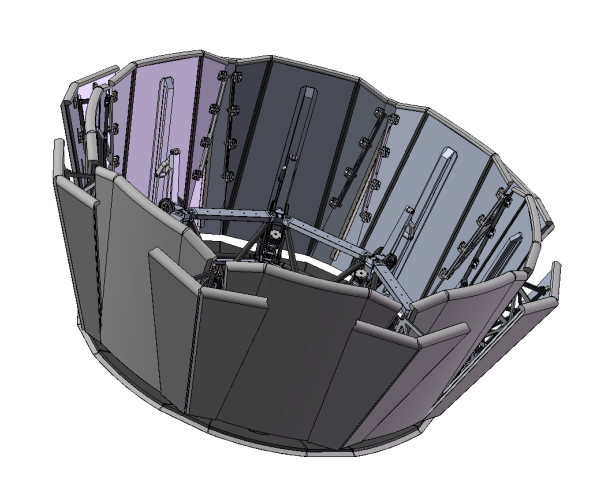
\includegraphics[width=\textwidth]{../Images/1. Introduction/HathorStowed.png}
        \caption{Deployed configuration.}
    \end{subfigure}
    \hfill
    \begin{subfigure}{0.56\textwidth}
        \centering
        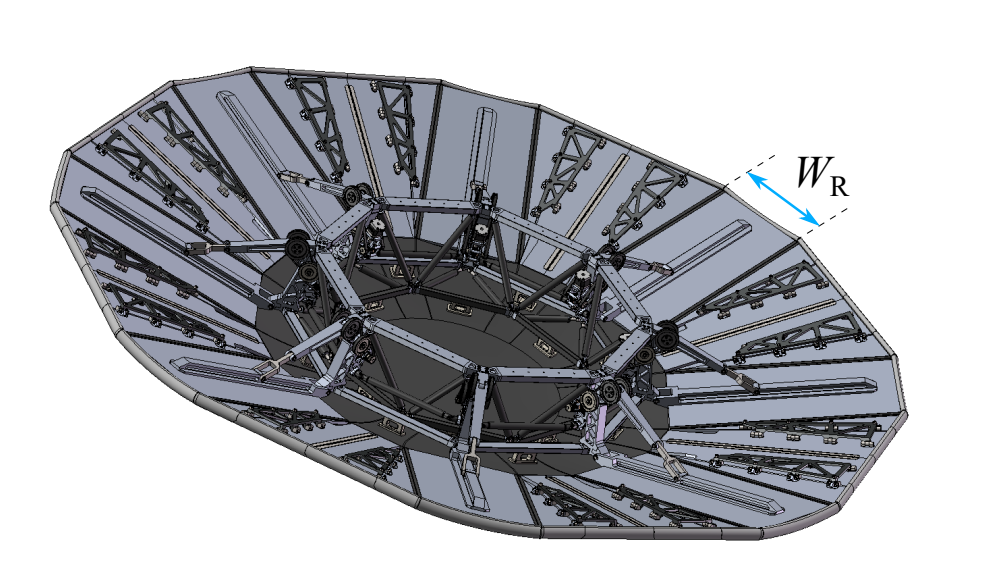
\includegraphics[width=\textwidth]{../Images/1. Introduction/HathorDeployed.png}  
        \caption{Stowed configuration.}
    \end{subfigure}
    \caption{Sketches of HATHOR \cite{hathoraero1}.}
    \label{fig:hathorsketch}
\end{figure}

This aerothermal analysis was conducted using both HEAT-3D \cite{heat3d}, a reduced order model for rapid prototyping of thermal protection systems \cite{hathoraero1}, and wind tunnel experiment paired with a coupled heat transfer CFD simulation \cite{hathoraero2}. 
In the latter, notable discrepancies emerged between the physical experiment and the simulation. These discrepancies sparked a discussion, which highlighted the possibility that they might be caused by rarefied flow, a condition known to impact aerodynamic properties. 

The combination of this intriguing intuitions and their relevance in the aforementioned situation of heightened interest into space exploration served as the primary motivation behind the research presented in this thesis. The foucs of this study revolves around exploring heat transfer in simple bodies under hypersonic rarefied conditions, particularly focusing on sharp corners, with the aims of investigating the evolution of Stanton number in rarefied flow and determining a correction factor to be used in codes for rapid aerothermal prototyping, such as HEAT-3D.

In \autoref{section:2} the theoretical background behind rarefied flow will be investigated and relevant research about its modelling will be presented.

Section \ref{section:3} will outline the general principles of operations of a Direct Simulation Monte Carlo code, which will subsequently be used to design and validate four set of simulations: varying global Knudsen number, varying edge radius, constant local Knudsen number and varying angle of attack. a full set of convergence studies will also be conducted, in order to ensure the accuracy of the simulatons.

The main findings of the research will thus be outlined and discussed in \autoref{section:4}.


\newpage

\section{Theoretical background and literature review}
\label{section:2}

\subsection{Rarefied flow}
The expression rarefied flow refers to a set of flow conditions where the gas is so rarefied that the continuum assumption of ordinary fluid mechanics ceases to be valid \cite{aerothermonotes}. Because of this, statistical mechanics has to be employed to describe it, rather than continuum mechanics.

It is possible to determine whether a flow is rarefied through the Knudsen number, a dimensionless number defined as in \autoref{eq:knudsen}, where $\lambda$ is the mean free path of the flow molecules and $l$ is a characteristic length of the flow.
\begin{equation}
    Kn=\frac{\lambda}{l}
    \label{eq:knudsen}
\end{equation}
As it is possible to see from \autoref{fig:regimes}, flows can be divided into three categories based on Knudsen number:
\begin{figure}[ht]
    \centering
    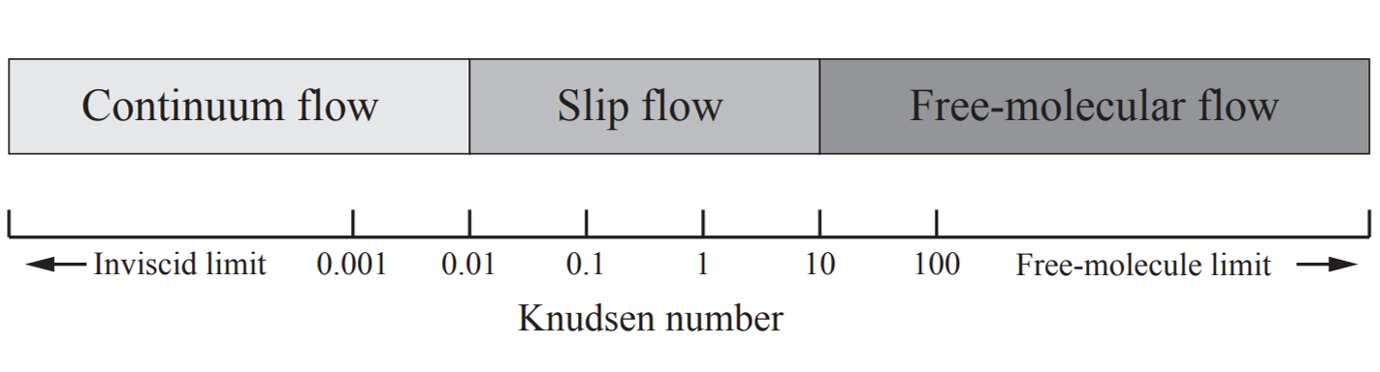
\includegraphics[width=0.7\textwidth]{../Images/2. Background/regimes.png}
    \caption{Flow regime with varying Knudsen number \cite{aerothermonotes}.}
    \label{fig:regimes}
\end{figure}
\begin{itemize}
    \item For Knudsen numbers below 10\textsuperscript{-2}, the flow can be classified as continuum. This kind of flow is characterised with a very significant number of intermolecular collision \cite{aerothermonotes, chambrerarefied}, and is commonly observed in everyday conditions, such as the flow around the wing of an aircraft or the flow of water in a pipe. It can be mathematically modelled through the Navier-Stokes equations.
    \item For Knudsen numbers between 10\textsuperscript{-2} and 10\textsuperscript{1}, flow can be classified as slip. In this condition the number of collisions between molecules is low, but not negligible \cite{chambrerarefied}. This leads to notable phenomena such as the boundary temperature jump, where the flow temperature at the wall differs from the surface wall temperature \cite{slipjump}. Moreover, a boundary slip velocity condition arises, which negates the the no-slip condition observed in ordinary flows \cite{slipjump}. These phenomena are schematically represented in \autoref{fig:slipjump}. The modelling of this regime depends on $Kn$. For conditions which approach the continuum flow, this regime can be modeled by incorporating correction factors into the Navier stokes equations \cite{slipjump} (in order to account for the aforementioned phenomena). Alternatively, it can be described through the Burnett and super Burnett equations \cite{burnett}.
    \item For Knudsen numbers above 10\textsuperscript{1}, the flow is classified as free molecular flow. In this regime, intermolecular collisions are so rare that the notion of an ordered flow of molecules ceases to exist \cite{aerothermonotes, chambrerarefied}, and is replaced by a statistical description, in the form of the Boltzmann equation, which can be seen in 
\end{itemize}
\begin{figure}[ht]
    \centering
    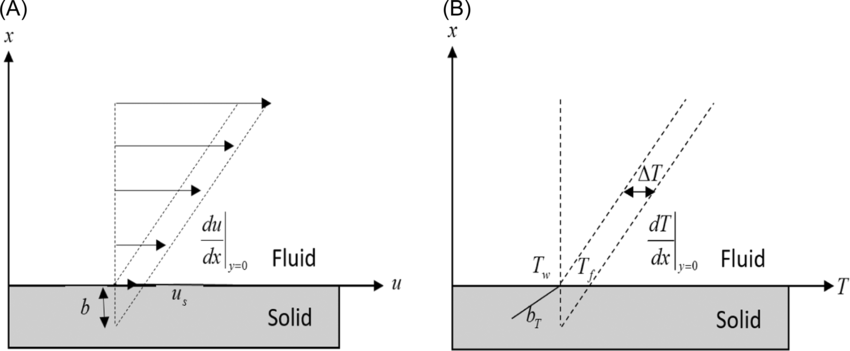
\includegraphics[width=0.7\textwidth]{../Images/2. Background/slipjump.png}
    \caption{Schematic diagram of velocity slip (A) and temperature jump (B)  \cite{slipjump}.}
    \label{fig:slipjump}
\end{figure}

It is important to note that while a flow may be globally continuous, certain local regions may exhibit signs of rarefied flow. An illustrative example of this phenomenon is the re-entry path of the space shuttle. While the global Knudsen number, calculated based on the length of the vehicle, may fall within the continuum regime, the Knudsen number associated with the flow around one of the rivets on its wing could differ significantly, potentially resulting in a different flow regime altogether.




\newpage

\section{Methodology}
\subsection{Direct Simulation Monte Carlo method}
The Direct Simulation Monte Carlo method  was initially introduced by Graeme A. Bird in the 1960s, and has become with time the de facto standard for rarefied flow simulations. When it was first developed, this method represented a radical departure from the traditional approaches employing a mathematical description of the flow, to such an extent that many questioned the validity of its results. It was eventually proven though, that, for time step and cell size tending to zero, the DSMC method converges to a solution of the Boltzmann equation \cite{bird}.

This method models the gas as a large collection of simulated particles, each representing an even wider set of real molecules. These molecules are propagated through the simulation domain, where they collide in a stochastic manner. \cite{themontecarlo}.

As the name in itself implies, this method is statistical at heart. Its results are in fact based on averaging the microscopic quantities of each of the molecules over a high number of time steps and over the grid cell size, in order to obtain global aerodynamic quantities. \cite{bird, themontecarlo}. This process will be discussed more in depth in \autoref{subsection:sampling}

\subsubsection{Particle description}
As mentioned previously, DSMC employs a particle description of the flow. The number of simulated particles is usually significantly lower than the real number of particles in the problem. This is due to the immense computational expense that simulating all of the particles in the real domain would require \cite{natodsmc}. To provide some perspective, it is useful to consider one of the most rarefied simulations conducted as part of this thesis. In this scenario, with a Knudsen number of 10 and a density of \SI{2e-7}{\kg\per\meter^3} (a mere 0.00001\% of the air density at sea level), more than \SI{3.6e18}{} molecules per cubic meter would have been required if a one-to-one correlation between the real and simulated molecules were to be maintained. The ratio between real and simulated molecules is expressed by $f_{num}$.

At the beginning of each simulation, a reference set of simulation particles is created. The microscopic properties (position and velocity) of each of the molecules in this set are chosen such that the bulk velocity and the global temperature of the flow correspond to the ones specified by the user, and that the number of simulated particles in the domain is equal to $\frac{n_{real}}{f_{num}}$. The velocity of the particles is usually selected through the Maxwell-Boltzmann distribution \cite{natodsmc}.

The simulated particles are not identical to the real particles: to correctly simulate the behaviour of the system the radius of each simulated particle must be proportional to the number of real particles that it represents, and is thus calculated such that \autoref{eq:radius} is valid. This approach also ensures the correct number of collisions in the flow \cite{dsmcnotes}.
\begin{equation}
    n_{real}\, \sigma_{real} = n_{sim}\, \sigma_{sim}
    \label{eq:radius}
\end{equation}
No indication of how the mass of each of the simulated particles is determined has been found in literature. However, based on how the SPARTA DSMC code calculates surface quantities, it is the author's understanding that the mass of the simulated particles is equal to the mass of the real particles.

\subsubsection{Mesh}
The DSMC method discretises the domain into a collection of mesh elements. This might seem counter intuitive, as the method operates on a particle-based description of the flow, which does not require the solution of any partial differential equation.

The mesh discretisation serves two main purposes: 

\begin{itemize}
    \item It allows to reduce the computational expense: employing pure Newtonian mechanics for all the molecules within the simulation domain would be too computationally expensive \cite{themontecarlo}. Thus DSMC only computes collision of randomly selected molecules within the same cell, disregarding collisions between molecules belonging to different cells, significantly cutting the computational burden. This topic will be discussed in more detail in \autoref{subsection:collision}
    \item It allows the calculation of global quantities such as temperature, bulk flow velocity or density by averaging the microscopic properties of the simulated particles over the cell volume. More details about this process can be found in section \autoref{subsection:sampling}.
\end{itemize}

As an added benefit, discretising the domain allows to parallelise the code by assigning chunks of cells of each processor, thus lowering the time required for the simulation.

\subsubsection{Boundary conditions}
One of the main advantages of the DSMC method is the ease of computing and assigning boundary conditions. Generally speaking, five boundary conditions exist \cite{natodsmc, spartadoc}
\begin{itemize}
    \item Outflow boundary: particles that cross this boundary are removed from the simulation.
    \item Inflow boundary: this type of boundary acts as a reservoir with gas properties specified in the simulation file. Particles are emitted into the simulation based on a surface generator (where the number of particles to be injected is determined from the number flux and their velocity from a surface distribution) or a volume generator (where a layer of "ghost cells" is created and filled with particles that satisfy the reference state properties, and the ones that do not cross the boundary after the particle move are discarded) \cite{natodsmc}. An inflow boundary also acts as an outflow boundary for particles that cross it from the simulation domain.
    \item Periodic boundary: the particles that cross this boundary exit the simulation and re-enter it at the opposite boundary (e.g., if the top of the simulation is a periodic boundary, particles will re-enter the simulation from the bottom) with unchanged velocity.
    \item Specular boundary: particles that cross this boundary reflect off of it with inverted normal velocity.
    \item Surface/thermal wall: particle that cross a surface are scattered based on the chosen surface-particle interaction model. More details will be given in \autoref{subsection:partsurf}.
\end{itemize}

\subsubsection{Particle motion}
Particles propagate through the simulation domain based on ordinary Newtonian mechanics. \autoref{eq:posupdate} shows the position update equation \cite{bird}, where $\mathbf{r}$ is the position vector of the particle, $\mathbf{v}$ is the velocity of the particle and $\Delta{t}$ is the time step.
\begin{equation}
    \Delta{\mathbf{r}} = \mathbf{v}\, \Delta{t}
    \label{eq:posupdate}
\end{equation}

\subsubsection{Particle collision selection}
\label{subsection:collision}
As previously mentioned, particle collisions are handled by DSMC with a probabilistic rather than deterministic approach. While it may seem intuitive to compute the trajectories of all the particles within a cell and check for collisions for each pair, or focus on nearby particles, DSMC takes a different approach.

In DSMC collision pairs are chosen at random, without taking into consideration their position or proximity to one another. A collision probability $P$, independent of the relative position of the molecules, is then computed, and the collision is said to happen with probability P \cite{bird, themontecarlo, natodsmc}.

The sequence of steps taken is the following:
\begin{enumerate}
    \item The number of candidate particles is computed based on \autoref{eq:candidate} \cite{themontecarlo}, where $N_{\mathrm{c}}$ is the number of particles in the cell, $\sigma$ is the collisional radius of the simulated molecules, $v_{\mathrm{r}, \max }$ is the maximum relative velocity and $V_{\mathrm{c}}$ is the cell volume.
    \begin{equation}
        N_{\mathrm{cand}}=\frac{N_{\mathrm{c}}^2\, \pi\, \sigma^2\, v_{\mathrm{r}, \max }\, f_{num}\, \Delta t}{2 V_{\mathrm{c}}}
        \label{eq:candidate}
    \end{equation}
    \item A pair of potential collision partners is randomly selected among the particles in the cell, and their collisional probability $P$ is computed. The collisional probability formula varies based on the chosen interaction model \cite{natodsmc}, but is usually proportional to both the collisional radius of the molecules and their relative velocity \cite{bird}.
    \item The pair is accepted as collision partners if their collision probability is higher than a random variable sampled from a uniform deviate in (0, 1) \cite{themontecarlo}.
    \item If the pair is accepted as collision partners, the new velocities of the molecules are computed and the algorithm moves to the next pair. Otherwise the algorithm moves to the next pair without modifying the velocities.
    \item The algorithm is repeated until the number of candidate particles is reached.
\end{enumerate}

\subsubsection{Intermolecular collision mechanics and models}
When particle collide with each other, their velocities are computed based on the chosen intermolecular collision model. All of the intermolecular collision models encountered in literature are partly based on momentum conservation, as in \autoref{eq:momcons}. The extra equations are derived based on the specific collision model
\begin{equation}
    m_{1,i}\; v_{1,i} + m_{2,i}\; v_{2,i} = m_{1,f}\; v_{1,f} + m_{2,f}\; v_{2,f}
    \label{eq:momcons}
\end{equation}
The three most commonly employed models are:
\begin{itemize}
    \item Hard sphere model: this model treats molecules as impenetrable hard spheres with fixed collision diameter. Velocities are computed based on elastic collision theory \cite{collisionmodels}.
    \item Variable hard sphere (VHS) model: this model is based on the hard sphere model, but it expands it by considering a variable collision diameter, based on the particle relative velocity. Post collision velocities are again determined based on elastic collision theory. This method resulted in scattering which was in poor agreement with the experimental results, which led to the development of the variable soft sphere model \cite{collisionmodels}.
    \item Variable soft sphere (VSS) model: this model introduces an extra parameter $\alpha$, which governs the post collision scattering of the particles (which becomes anisotropic) \cite{collisionmodels}.
\end{itemize}

Many more models exist, such as the Generalized Hard Sphere (GHS) or Lennard-Jones (L-J) models \cite{collisionmodels}, but they are beyond the scope of this dissertation.

\subsubsection{Particle-surface interactions}
\label{subsection:partsurf}
As for particle-particle interactions, many models exist for particle-surface interaction. The two most commonly used ones are:
\begin{itemize}
    \item Specular reflection: this model reflects the particle with inverted normal velocity and unchanged parallel velocity. Since there is no change in velocity, no energy is transferred to the surface.
    \item Diffuse reflection: this model reflects the particles independently of their velocity before reflection. The post collision velocity is usually determined from a Maxwellian distribution based on the wall temperature \cite{bird, spartadoc}.
\end{itemize}

Many solvers allow to employ both the models at the same time through an accommodation coefficient, which determines what fraction of the collisions will be of each type.

More information about more advanced models can be found in \cite{spartadoc}.

\subsubsection{Sampling and calculation of global quantities}
\label{subsection:sampling}

To obtain useful global quantities from the microscopic properties of the molecules, a particle sampling is executed. This consists in determining the gas macroparameters by aggregating the molecular quantities of simulated particles and averaging them over the cell volume. 

\autoref{eq:density}, \autoref{eq:velocity}, and \autoref{eq:ke} respectively outline the mathematical process employed to execute the sampling for density, mass-weighted average u velocity, and average kinetic energy in the SPARTA DSMC code. In the aforementioned equations $f_{num}$ is the real to simulated particles ratio, $V_{\mathrm{c}}$ is the cell volume, $N_{\mathrm{c}}$ is the number of particles in the cell, $m_i$ is the mass of each particle and $u_i$, $v_i$, $w_i$, are respectively the $x$, $y$ and $z$ components of velocity.
\begin{equation}
    \rho = \frac{f_{num}}{V_{\mathrm{c}}}\; \sum_{i=1}^{N_{\mathrm{c}}}\; m_i
    \label{eq:density}
\end{equation}
\begin{equation}
    u = \frac{\sum_{i=1}^{N_{\mathrm{c}}}\; u_i\; m_i}{\sum_{i=1}^{N_{\mathrm{c}}}\; m_i} 
    \label{eq:velocity}
\end{equation}
\begin{equation}
    KE = \frac{1}{N_c}\; \sum_{i=1}^{N_{\mathrm{c}}}\; \frac{1}{2}\; m_i\; (u_i^2+v_i^2+w_i^2)
    \label{eq:ke}
\end{equation}
A similar procedure can be employed to get surface-specific values, such as the heat transfer or the force applied to a surface element.

Given the statistical noise inherent of a Monte Carlo method, the macroscopic quantities are also averaged over a number of time steps.

\subsubsection{Iterative procedure}
After 

\autoref{fig:dsmcflowchart} shows 

\begin{figure}[ht]
    \centering
    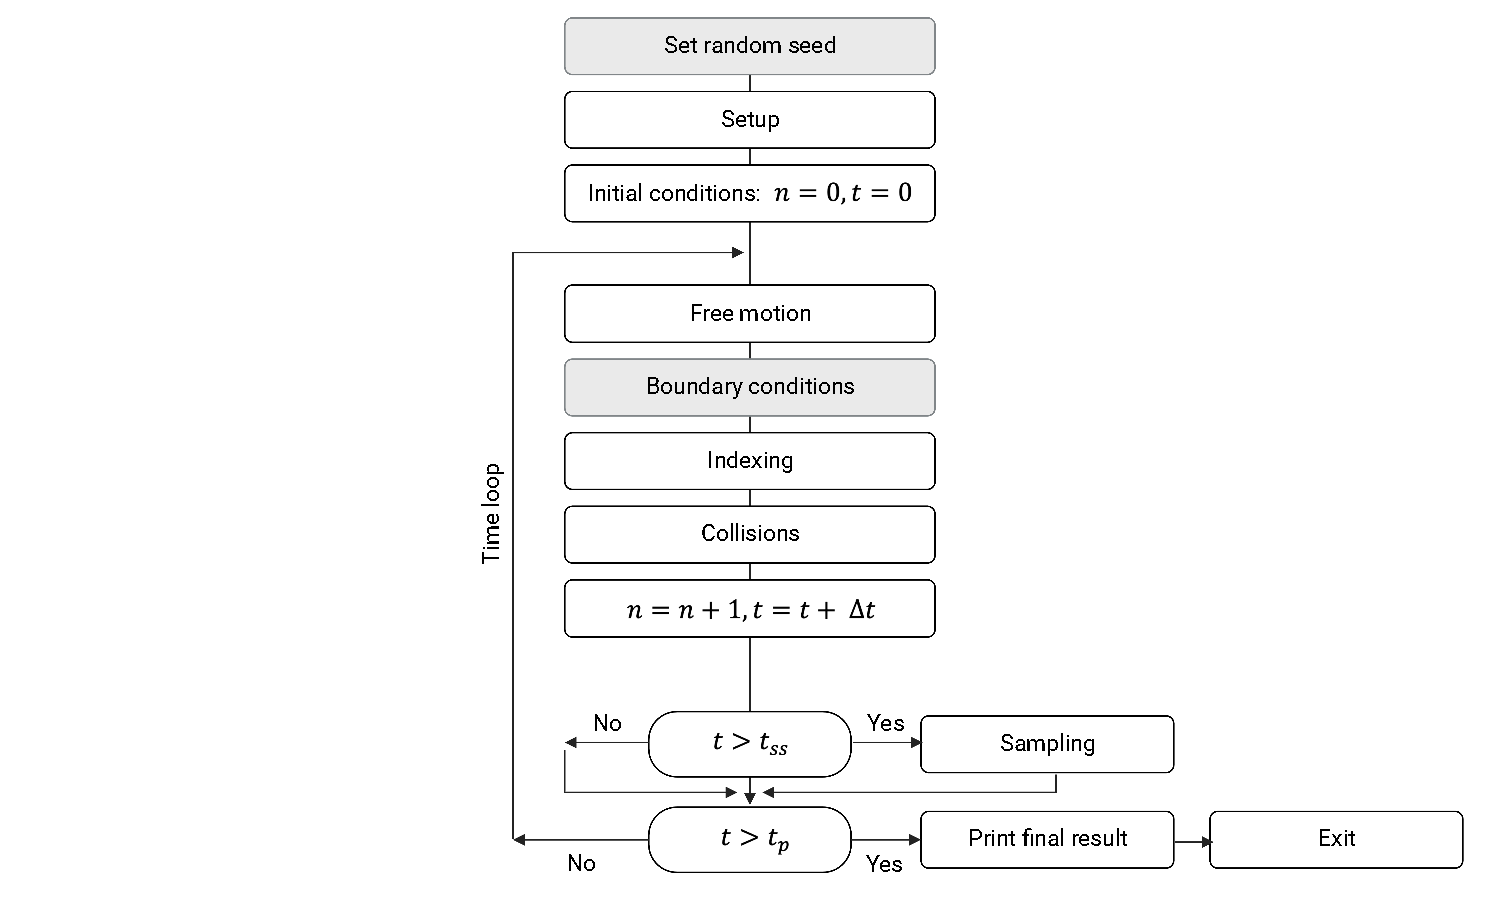
\includegraphics[width=\textwidth]{../Images/3. Methodology/dsmcflowchart.pdf}
    \caption{Flowchart of DSMC method loop. Adapted from \cite{dsmcnotes}.}
    \label{fig:dsmcflowchart}
\end{figure}
\newpage

\section{Results and discussion}
\label{section:4}

\subsection{Variation of global Knudsen number results}
\label{subsection:kn}

\autoref{fig:vcontoursquare} shows the velocity contour around a rounded corner square for varying values of Knudsen number.
\begin{figure}
    \centering
    \begin{subfigure}{0.32\textwidth}
        \centering
        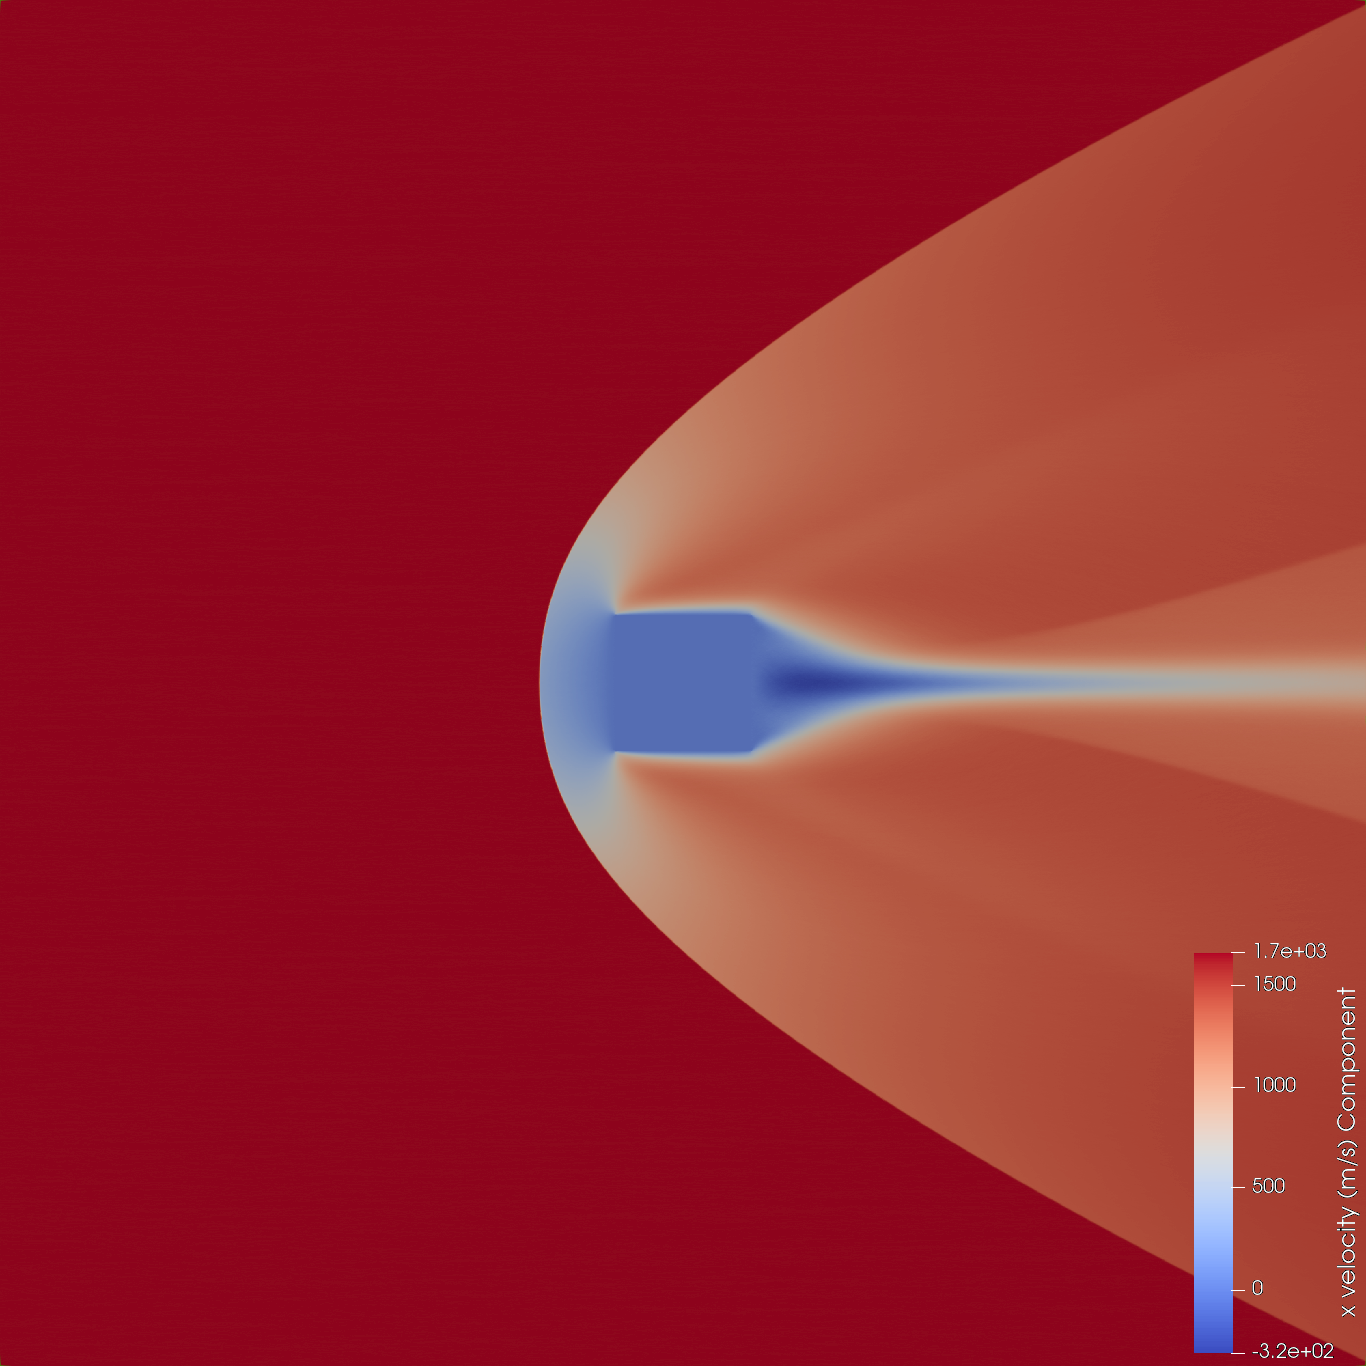
\includegraphics[width=\textwidth]{Images/4. Results/Square Kn/pv/Kn0.001.png}
        \caption{Kn = 0.001}
    \end{subfigure}
    \hfill
    \begin{subfigure}{0.32\textwidth}
        \centering
        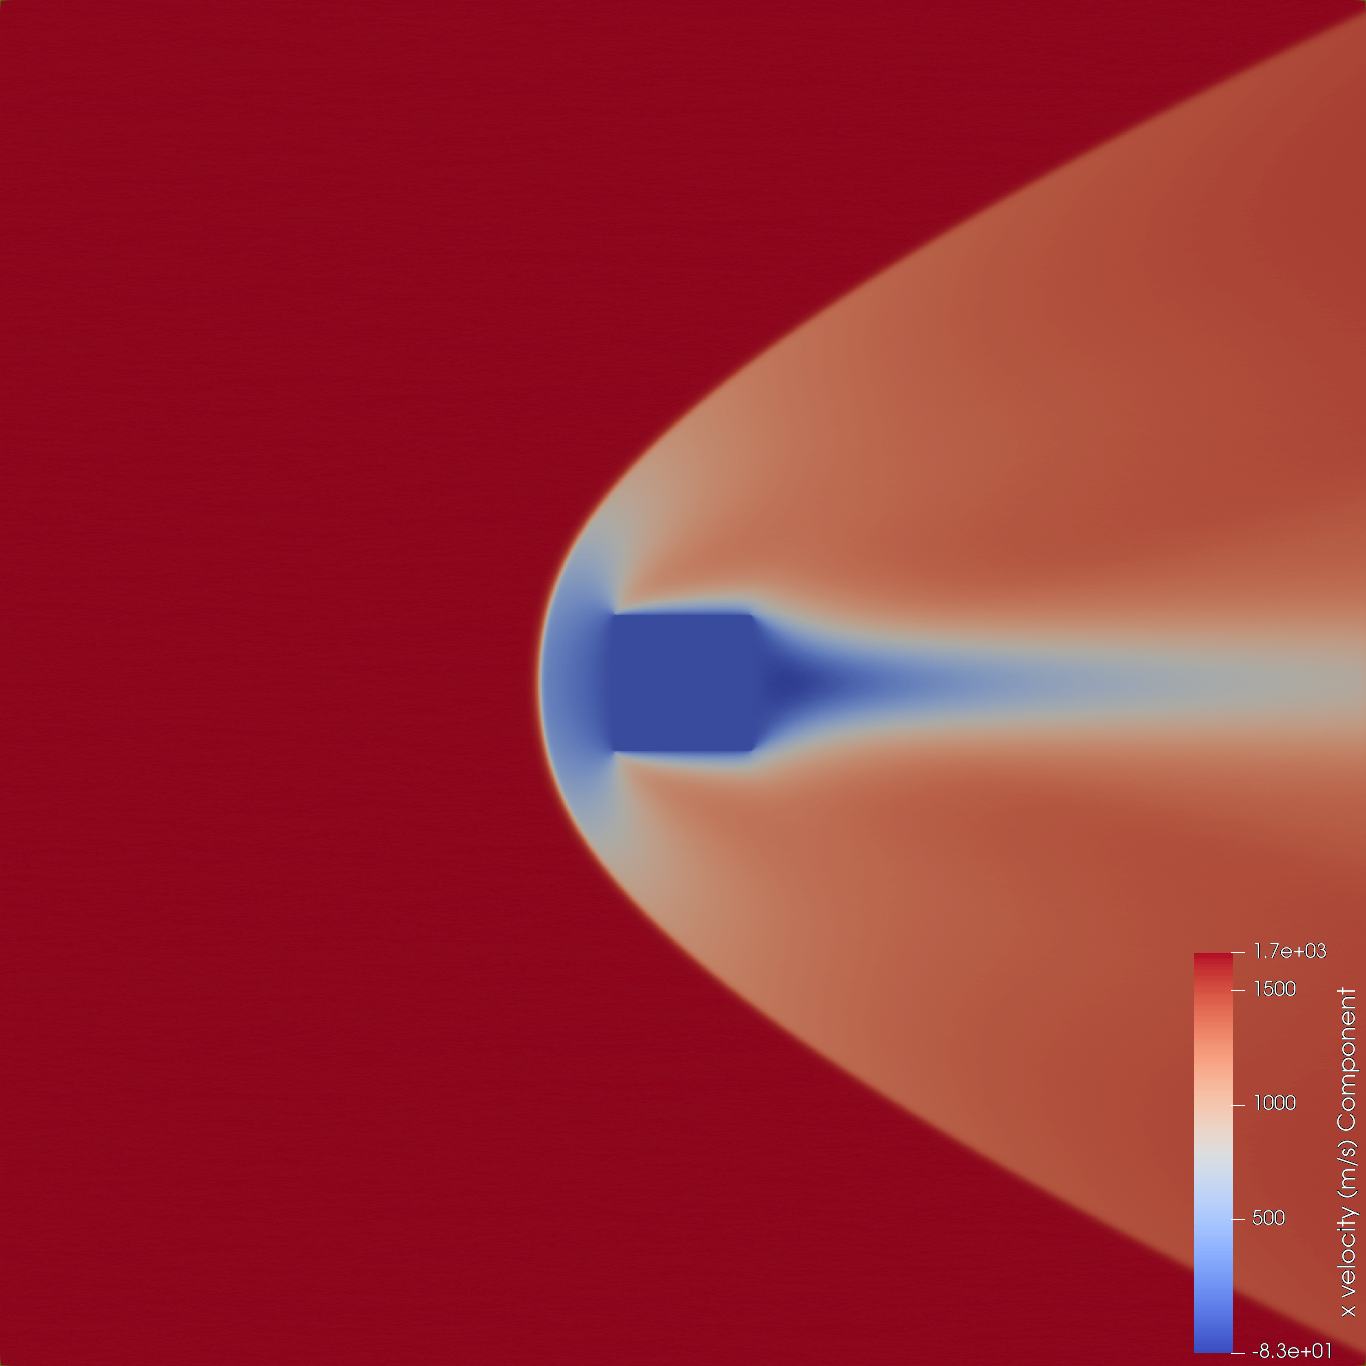
\includegraphics[width=\textwidth]{Images/4. Results/Square Kn/pv/Kn0.01.png}
        \caption{Kn = 0.01}
    \end{subfigure}
    \hfill
    \begin{subfigure}{0.32\textwidth}
        \centering
        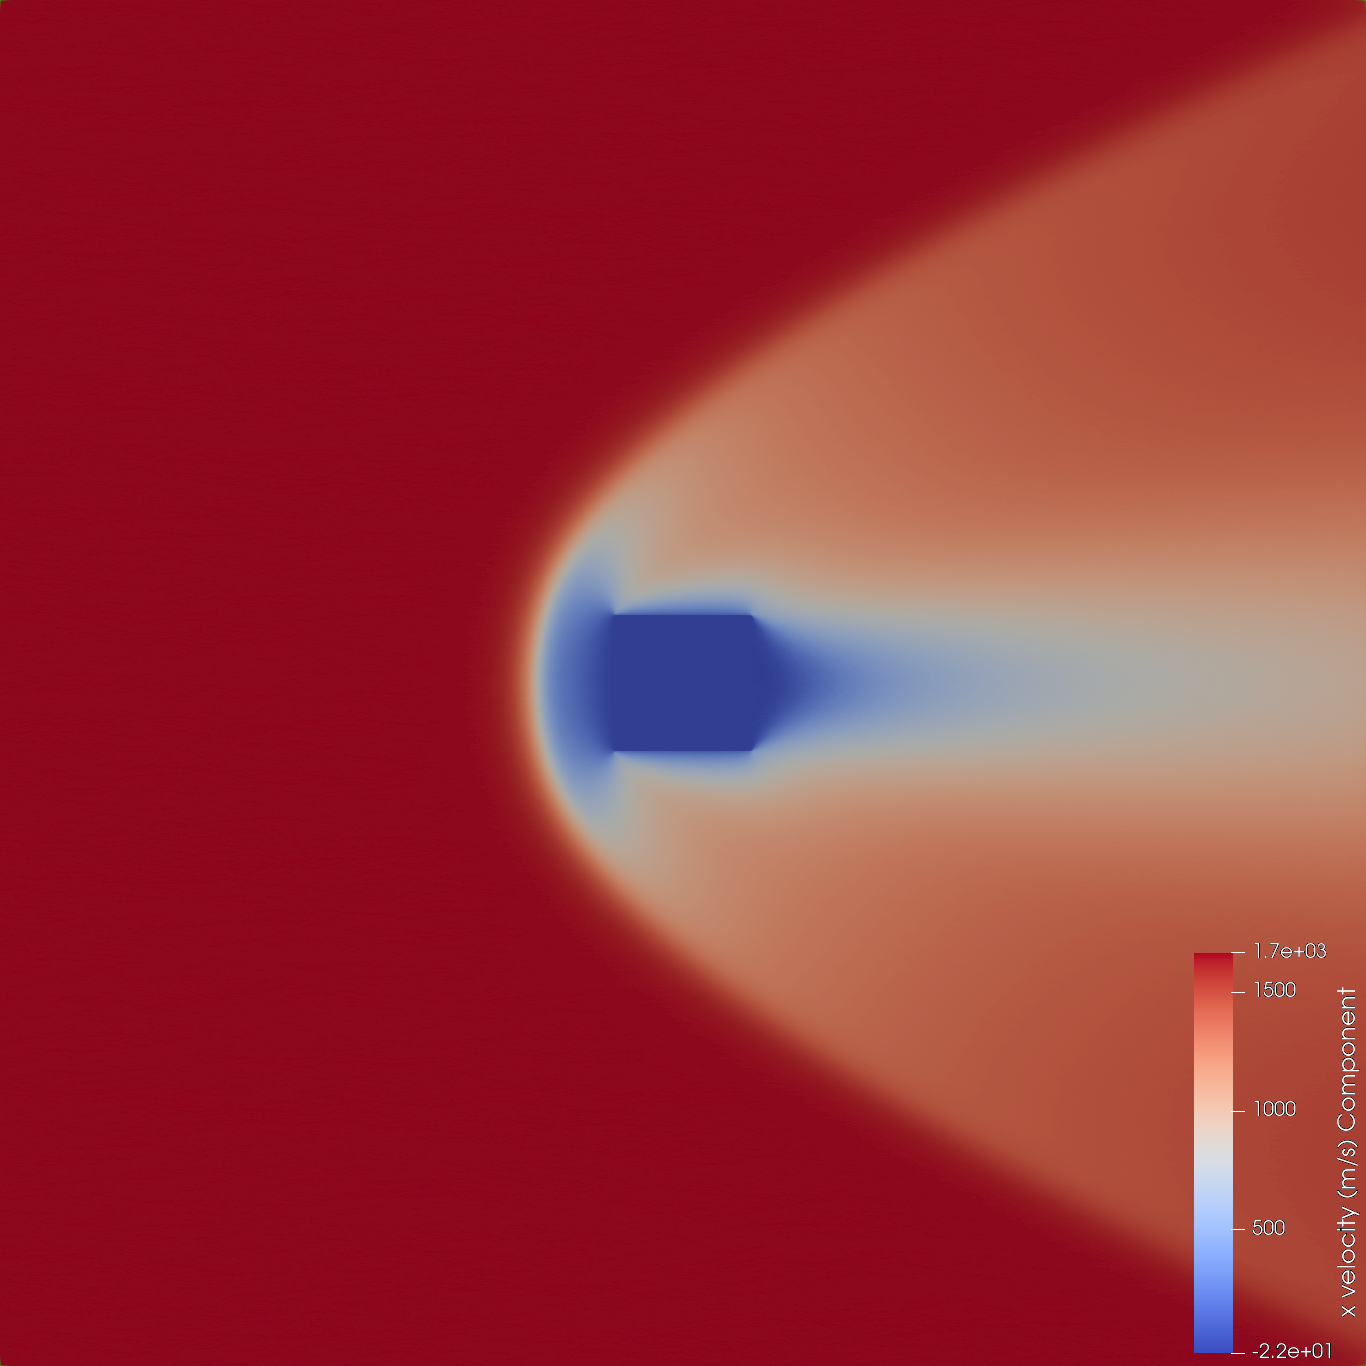
\includegraphics[width=\textwidth]{Images/4. Results/Square Kn/pv/Kn0.05.png}
        \caption{Kn = 0.05}
    \end{subfigure}
    
    \vspace{5pt}
    
    \centering
    \begin{subfigure}{0.32\textwidth}
        \centering
        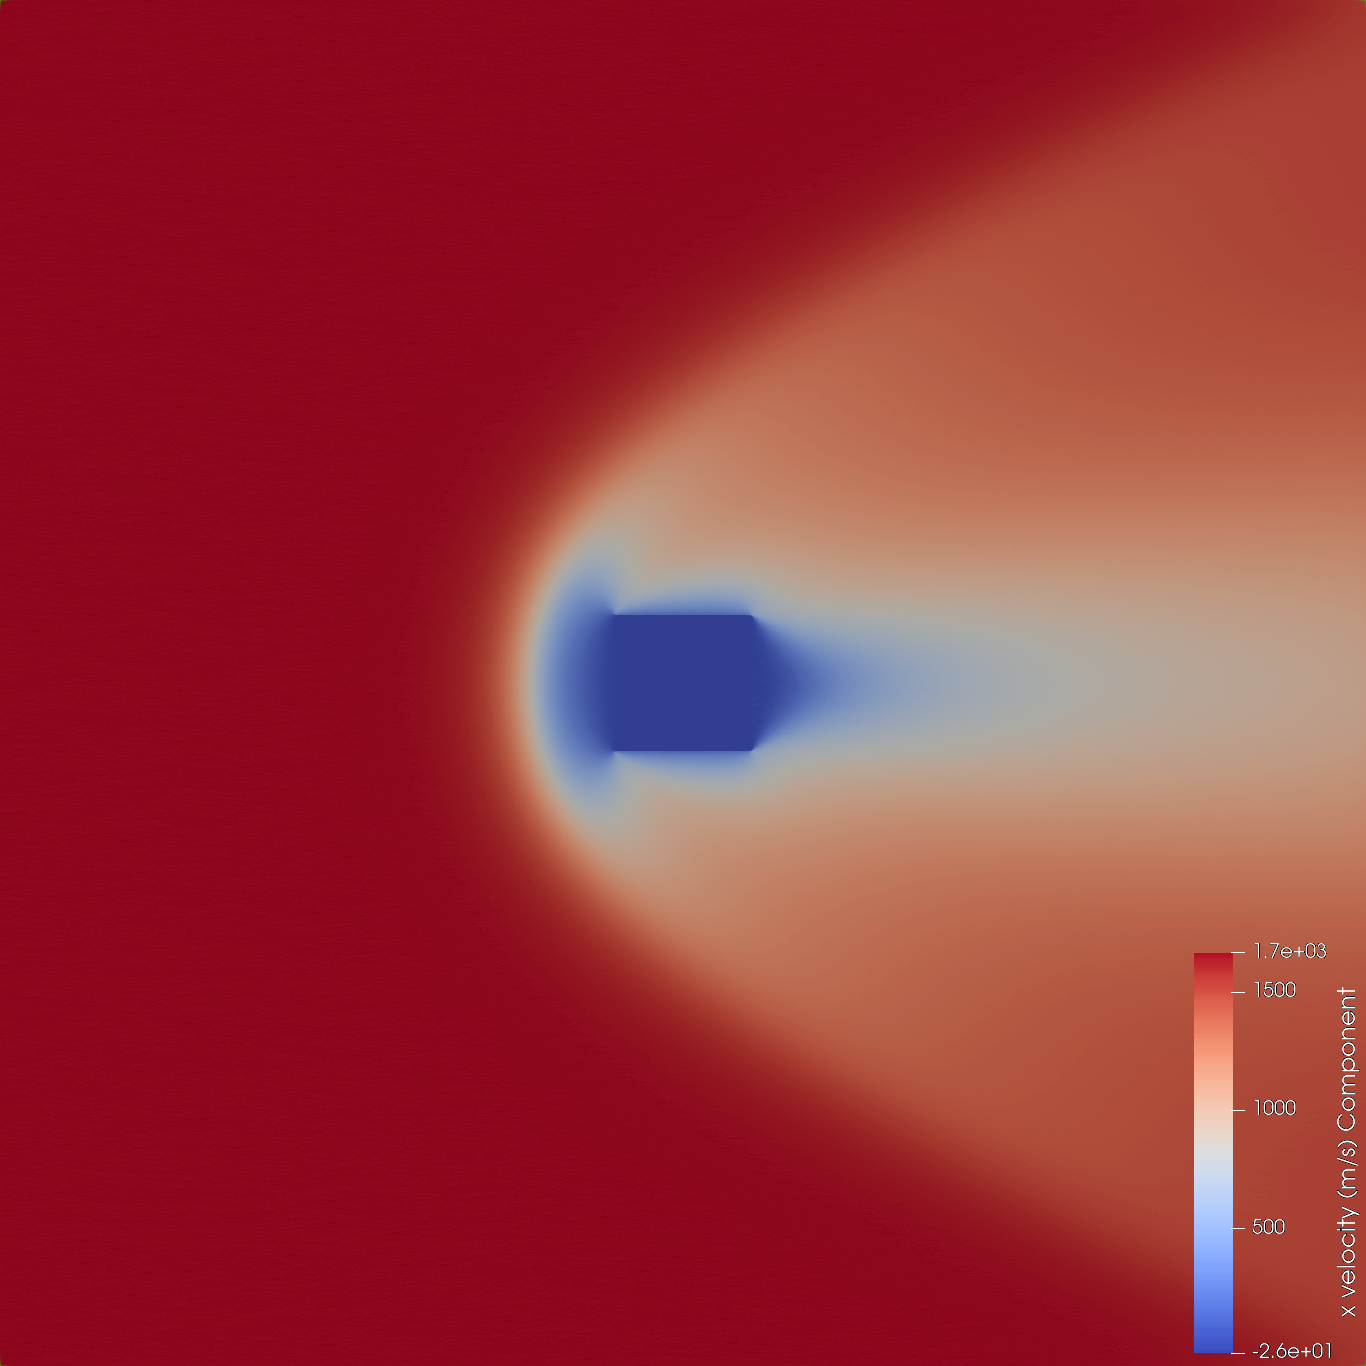
\includegraphics[width=\textwidth]{Images/4. Results/Square Kn/pv/Kn0.1.png}
        \caption{Kn = 0.1}
    \end{subfigure}
    \hfill
    \begin{subfigure}{0.32\textwidth}
        \centering
        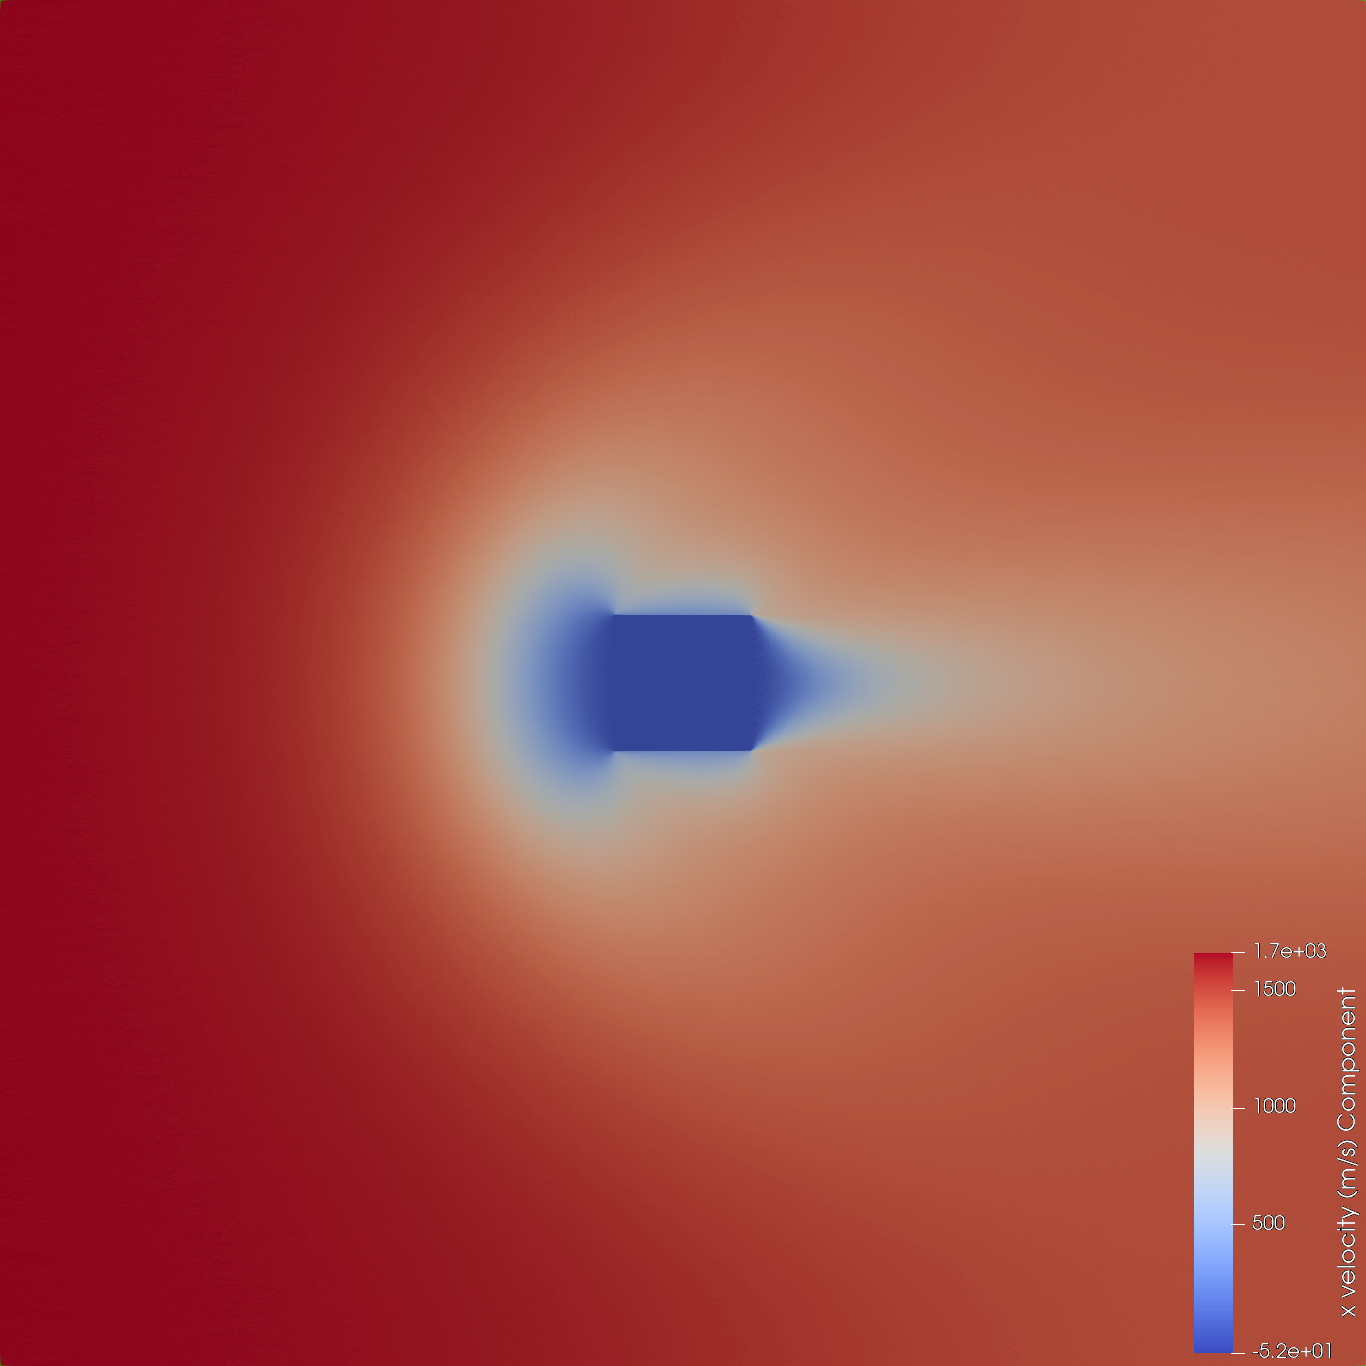
\includegraphics[width=\textwidth]{Images/4. Results/Square Kn/pv/Kn0.5.png}
        \caption{Kn = 0.5}
    \end{subfigure}
    \hfill
    \begin{subfigure}{0.32\textwidth}
        \centering
        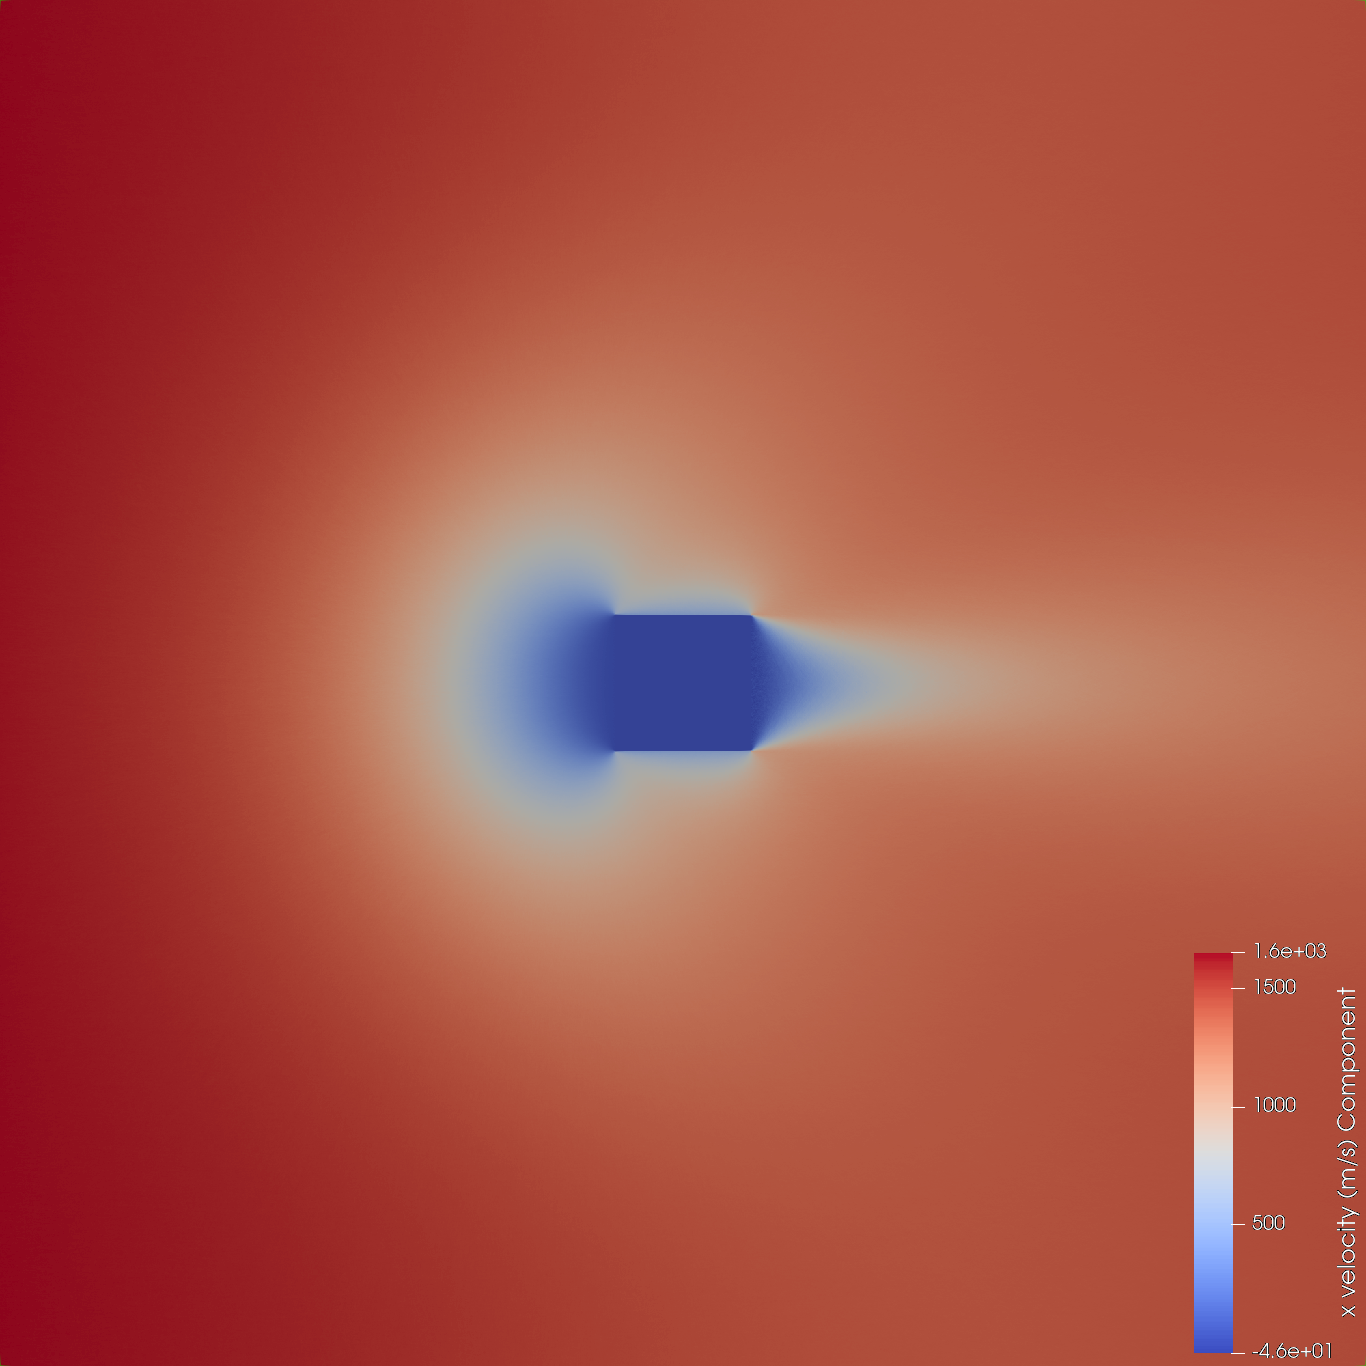
\includegraphics[width=\textwidth]{Images/4. Results/Square Kn/pv/Kn1.png}
        \caption{Kn = 1}
    \end{subfigure}
    
    \vspace{5pt}
    
    \centering
    \begin{subfigure}{0.32\textwidth}
        \centering
        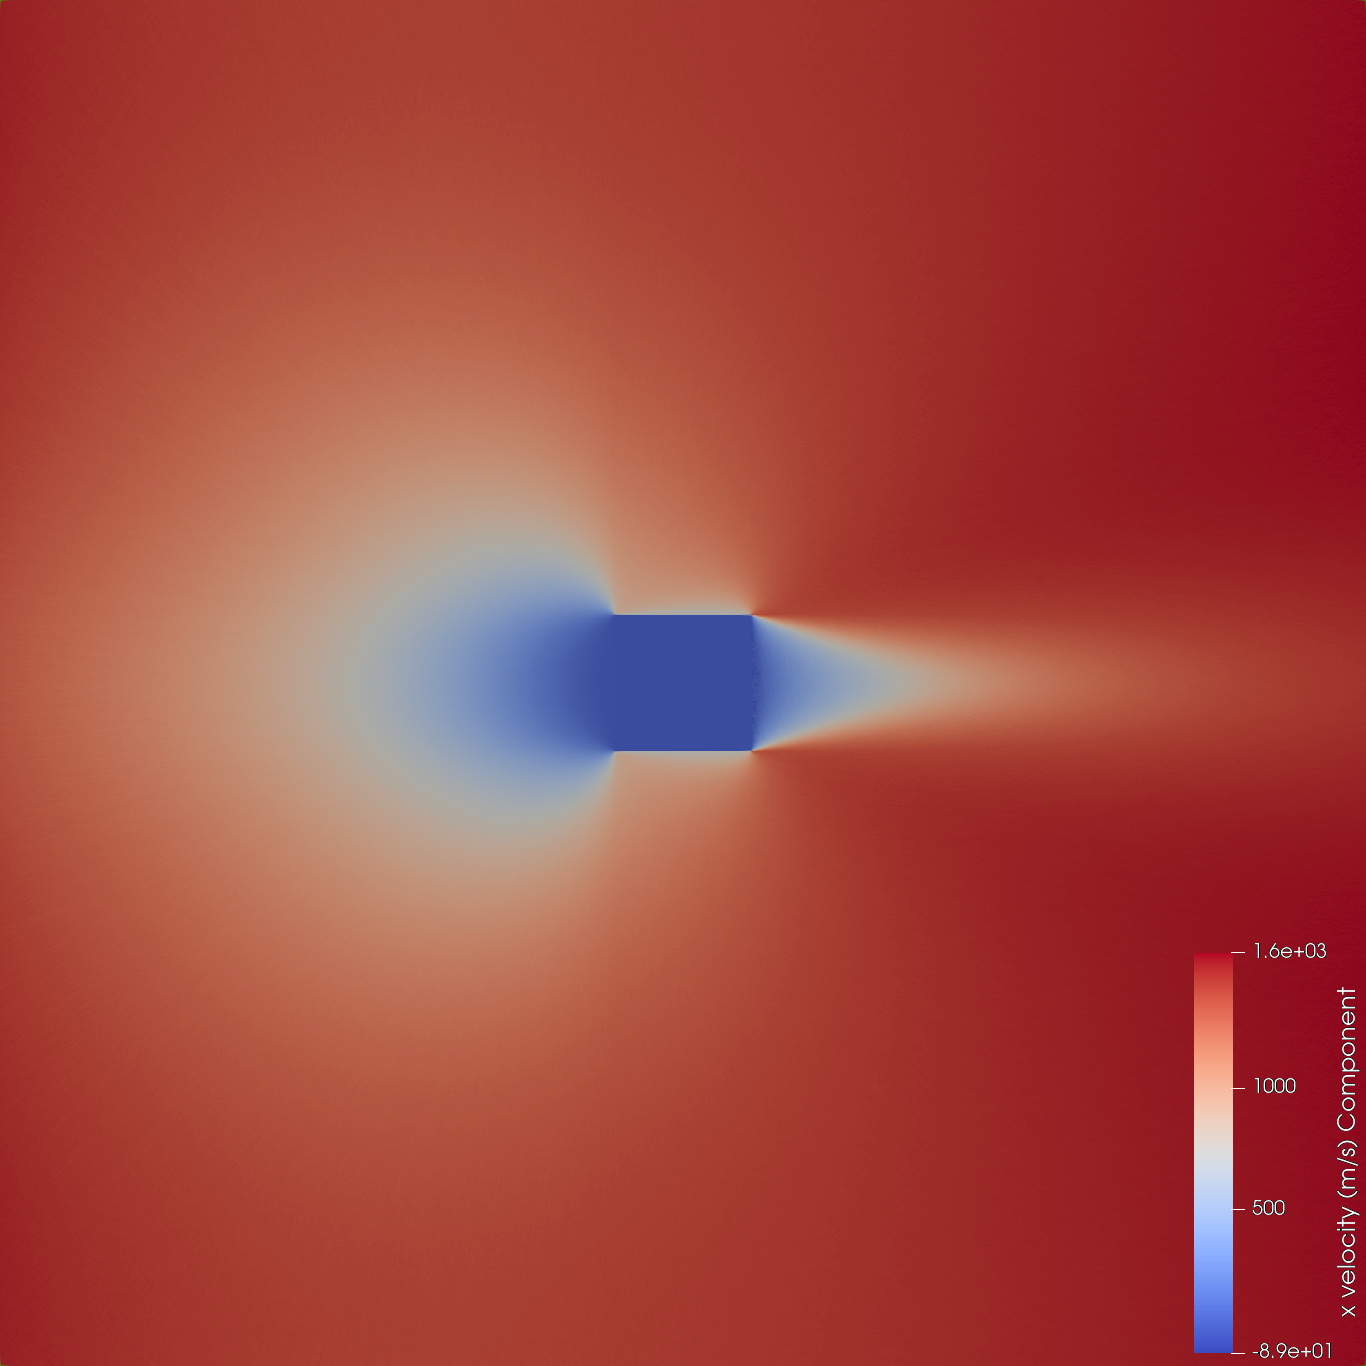
\includegraphics[width=\textwidth]{Images/4. Results/Square Kn/pv/Kn5.png}
        \caption{Kn = 5}
    \end{subfigure}
    \hfill
    \begin{subfigure}{0.32\textwidth}
        \centering
        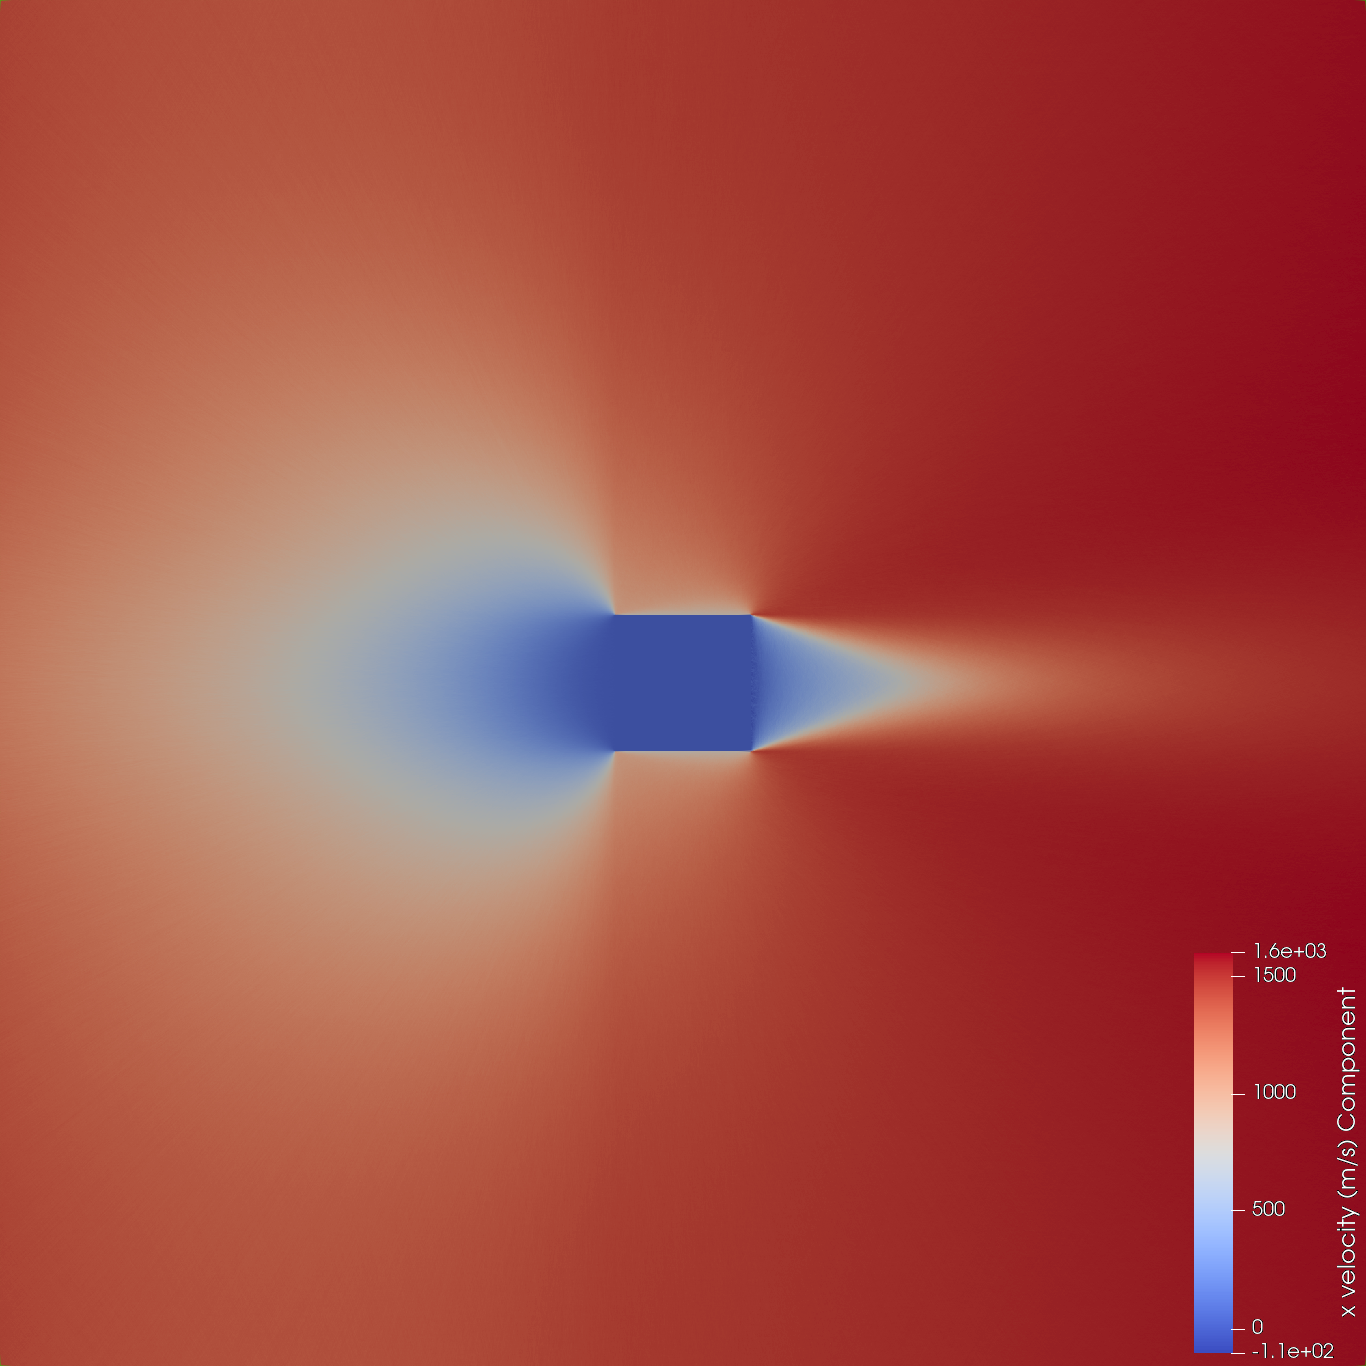
\includegraphics[width=\textwidth]{Images/4. Results/Square Kn/pv/Kn10.png}
        \caption{Kn = 10}
    \end{subfigure}
    \hfill
    \begin{subfigure}{0.32\textwidth}
        \centering
        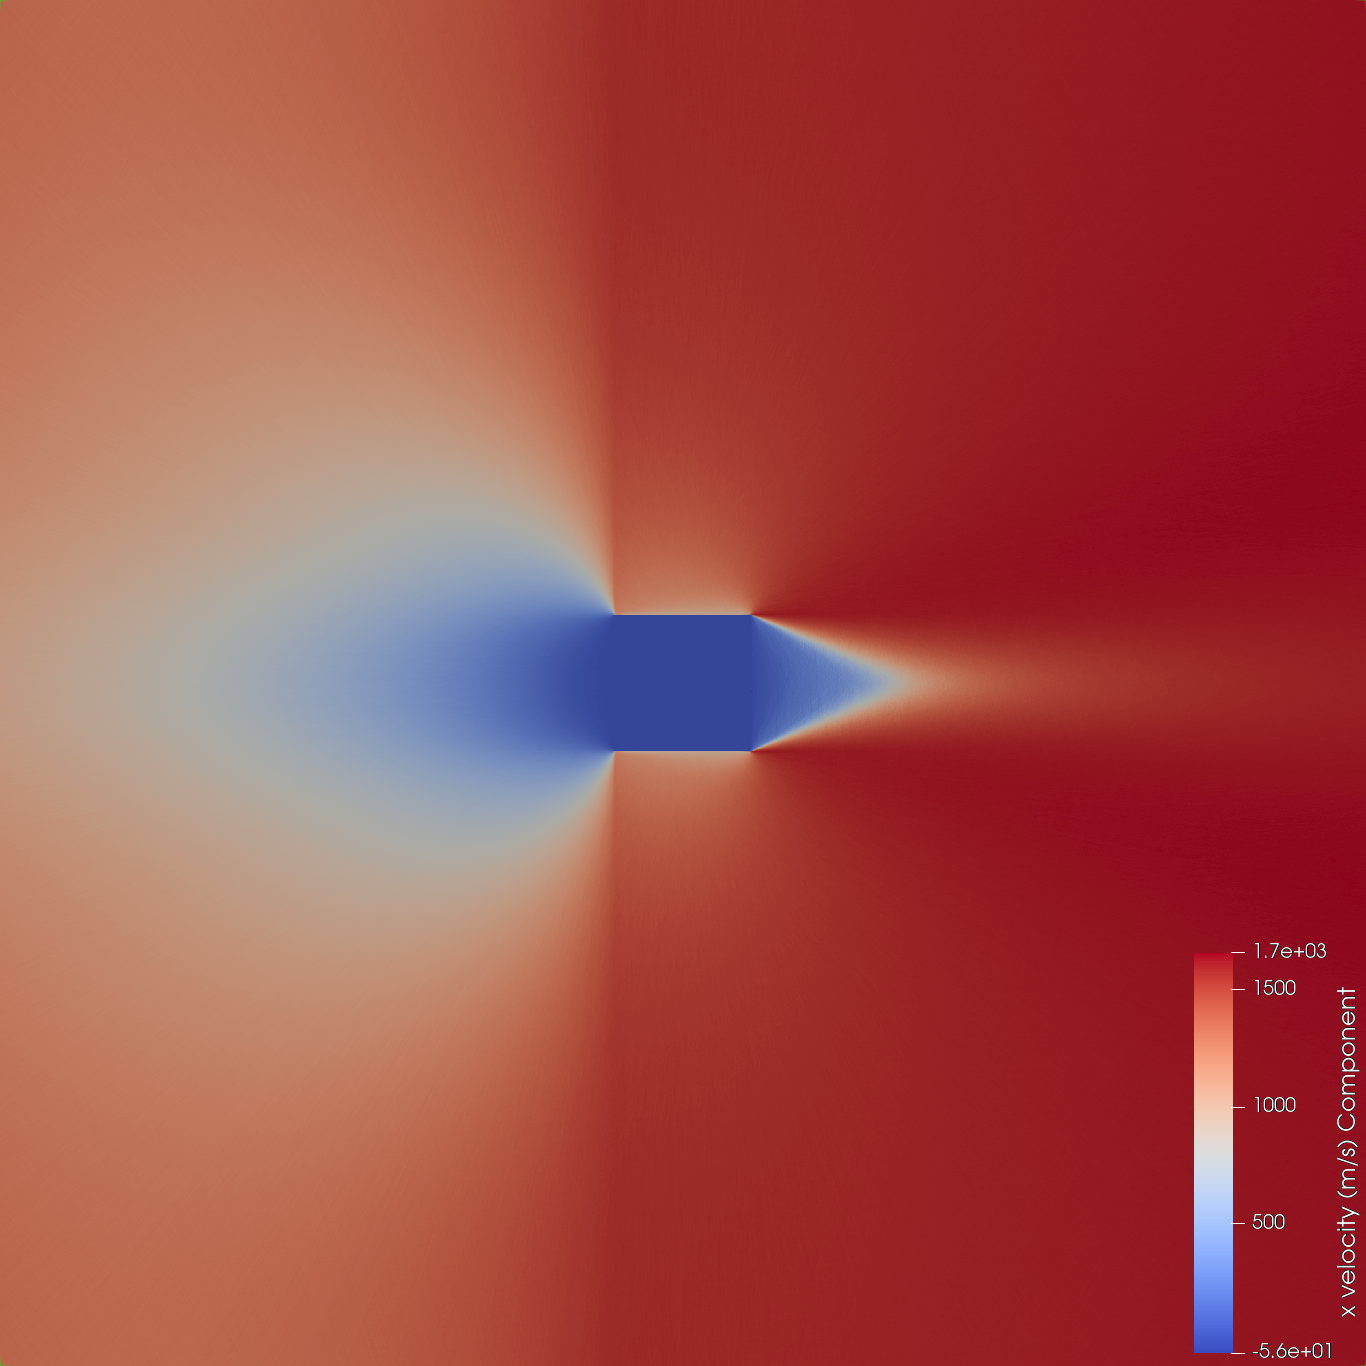
\includegraphics[width=\textwidth]{Images/4. Results/Square Kn/pv/Kn100.png}
        \caption{Kn = 100}
    \end{subfigure}
    \caption{Velocity contours around a rounded square for varying Knudsen number.}
    \label{fig:vcontoursquare}
\end{figure}

A radical change in flow conditions can be observed as the Knudsen number is increased. At a $Kn$ of 0.001, in the pure continuum regime, a number of classical features of supersonic flow can be pointed out: an instantaneous bow shock in front of the cube, expansion fans at its corners and two shocks generated by the expanded flow impinging on itself aft of it. As the Knudsen increased to 0.01 and then to 0.05, a gradual thickening of the boundary layer, typical of a decrease in Reynolds number can be spotted. Moreover, the expansion fans and the shock at the back become gradually less noticeable, and the instantaneous bow shock at the front starts to gradually smear. By $Kn = 0.1$, the shock has become very smeared, and the boundary layer has thickened by a very significant amount. Between the Knudsen numbers of 0.5 and 5, a drastic flow change occurs: the shockwave completely disappears, replaced by a zone of reduced velocity occupying the entire front section of the domain. As Knudsen number is increased even further, this effect becomes more evident, and a peculiar triangular structure (the origin of which his unknown)  appears in the wake of the cube.

This drastic change in flow behaviour could be explained with a paradigm shift in thought process: as mentioned many times, the flow based description of aerodynamics ceases to be valid at high Knudsen number, and it has to be replaced by a particle based one.

In the continuum regime, the flow impinging on the stagnation surface of the cube is forced to curve, first towards the corners and then around them. In a particle sense, when molecules that hit the surface of the cube are reflected in the opposite direction, they encounter other molecules that stop them from travelling against the flow and force them to curve. This produces a bow shock.
However, as the Knudsen number is increased (and thus the density falls), the number of particles forward of those that have just reflected off the surface decreases. Thus, a greater distance is necessary for particles travelling in the opposite direction to be redirected. This can be seen from \autoref{fig:pcontoursquare}.

At very high Knudsen numbers the "stopping effect" disappears almost entirely. Molecules that reflect off the stagnation surface are free to move in the opposite direction, effectively generating a second, completely separate flow.

The reduced velocity magnitude seen in front of the cube is thus probably an artefact, produced by the software as described in \autoref{eq:velocity} by averaging the velocity values of the particles belonging to the two flows over the cell area.

\begin{figure}
    \centering
    \begin{subfigure}{0.32\textwidth}
        \centering
        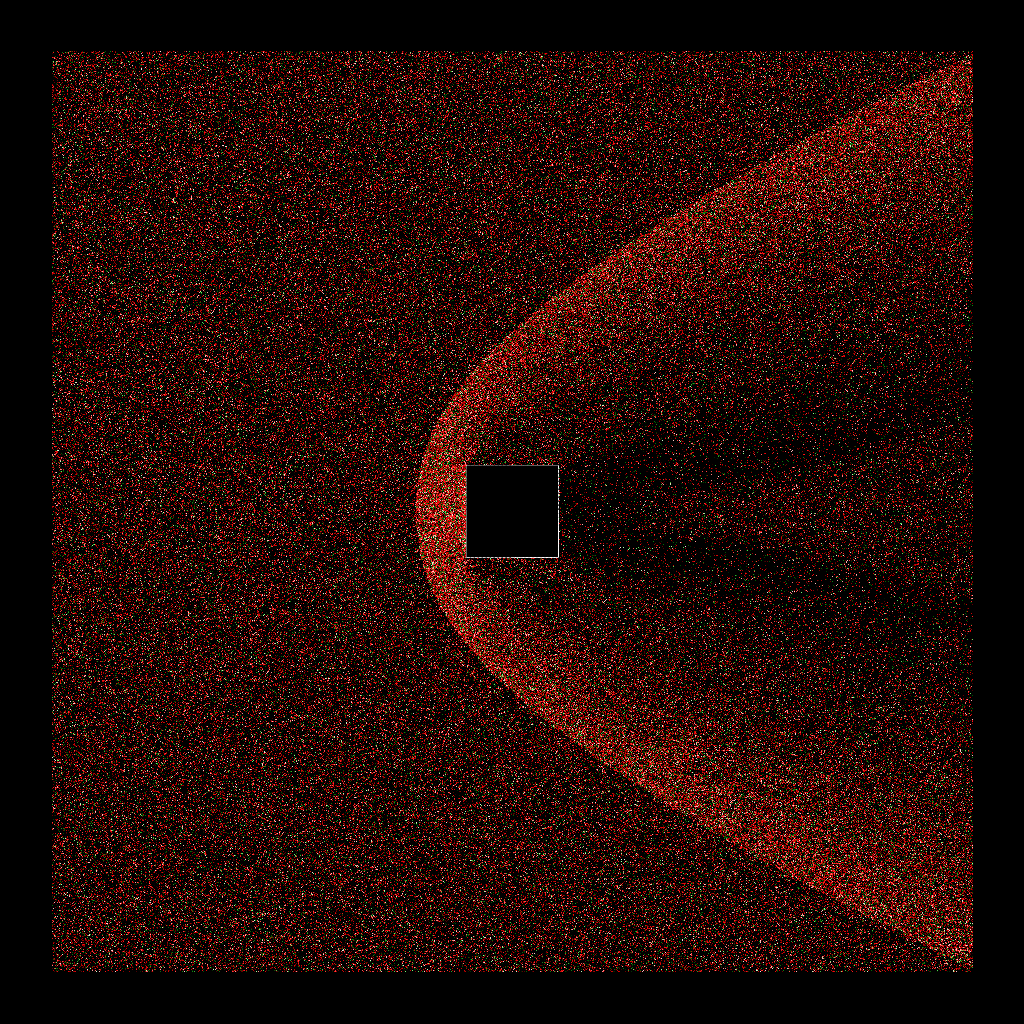
\includegraphics[width=\textwidth]{Images/4. Results/Square Kn/particles/Kn0.001.png}
        \caption{Kn = 0.001}
    \end{subfigure}
    \hfill
    \begin{subfigure}{0.32\textwidth}
        \centering
        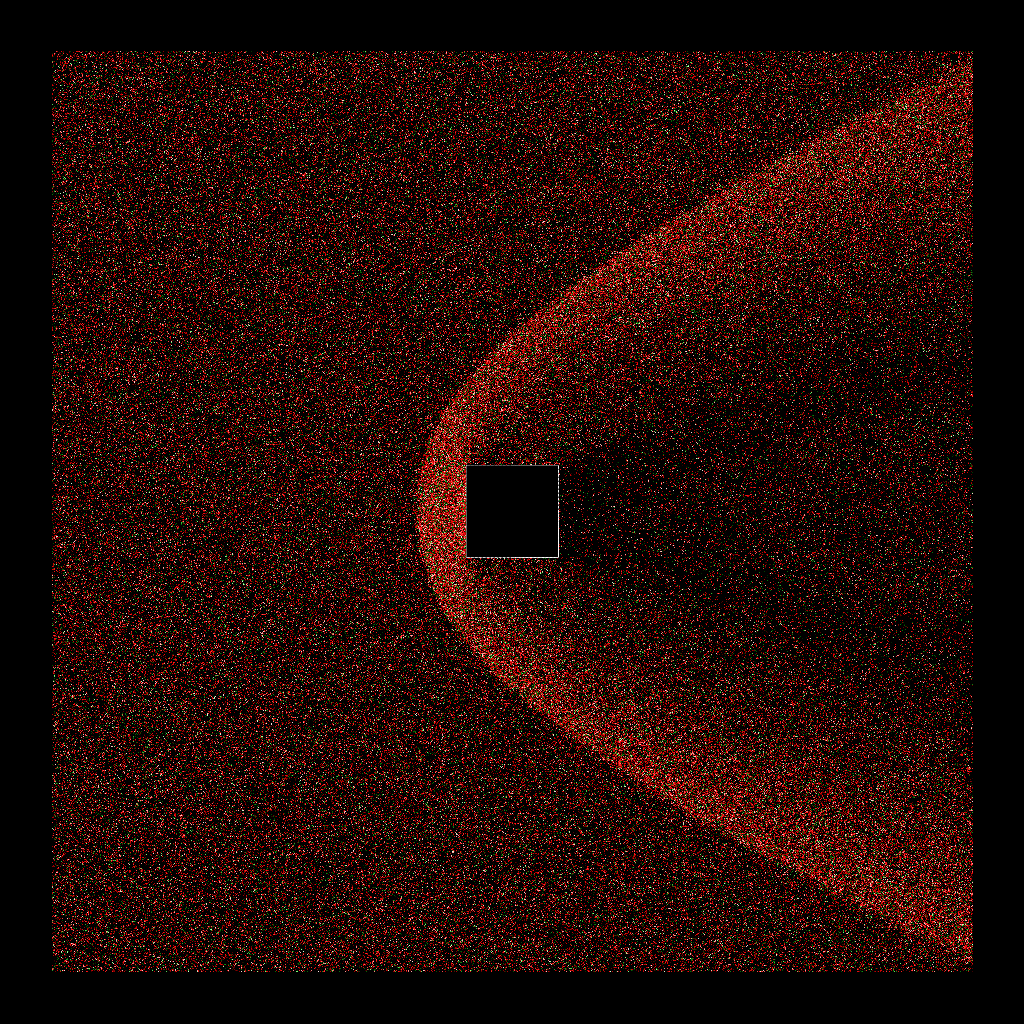
\includegraphics[width=\textwidth]{Images/4. Results/Square Kn/particles/Kn0.01.png}
        \caption{Kn = 0.01}
    \end{subfigure}
    \hfill
    \begin{subfigure}{0.32\textwidth}
        \centering
        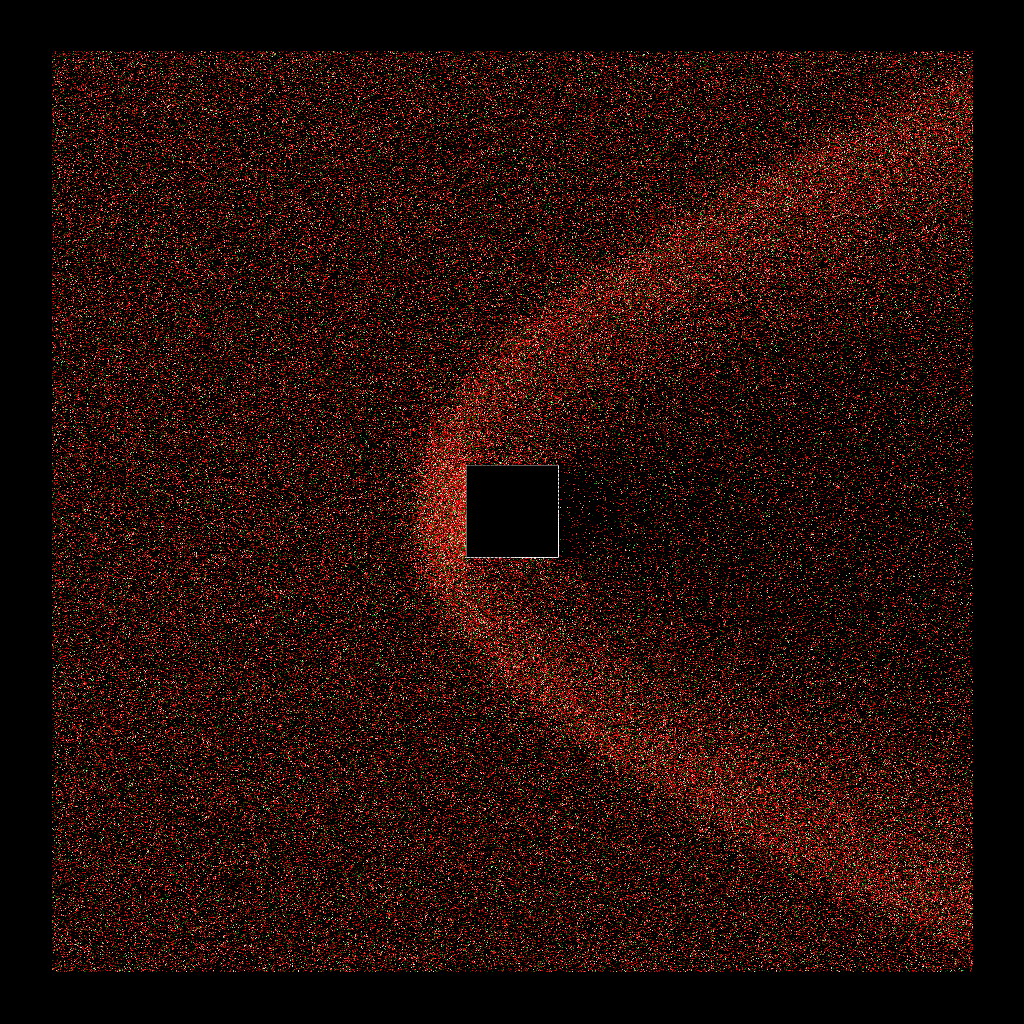
\includegraphics[width=\textwidth]{Images/4. Results/Square Kn/particles/Kn0.05.png}
        \caption{Kn = 0.05}
    \end{subfigure}
    
    \vspace{5pt}
    
    \centering
    \begin{subfigure}{0.32\textwidth}
        \centering
        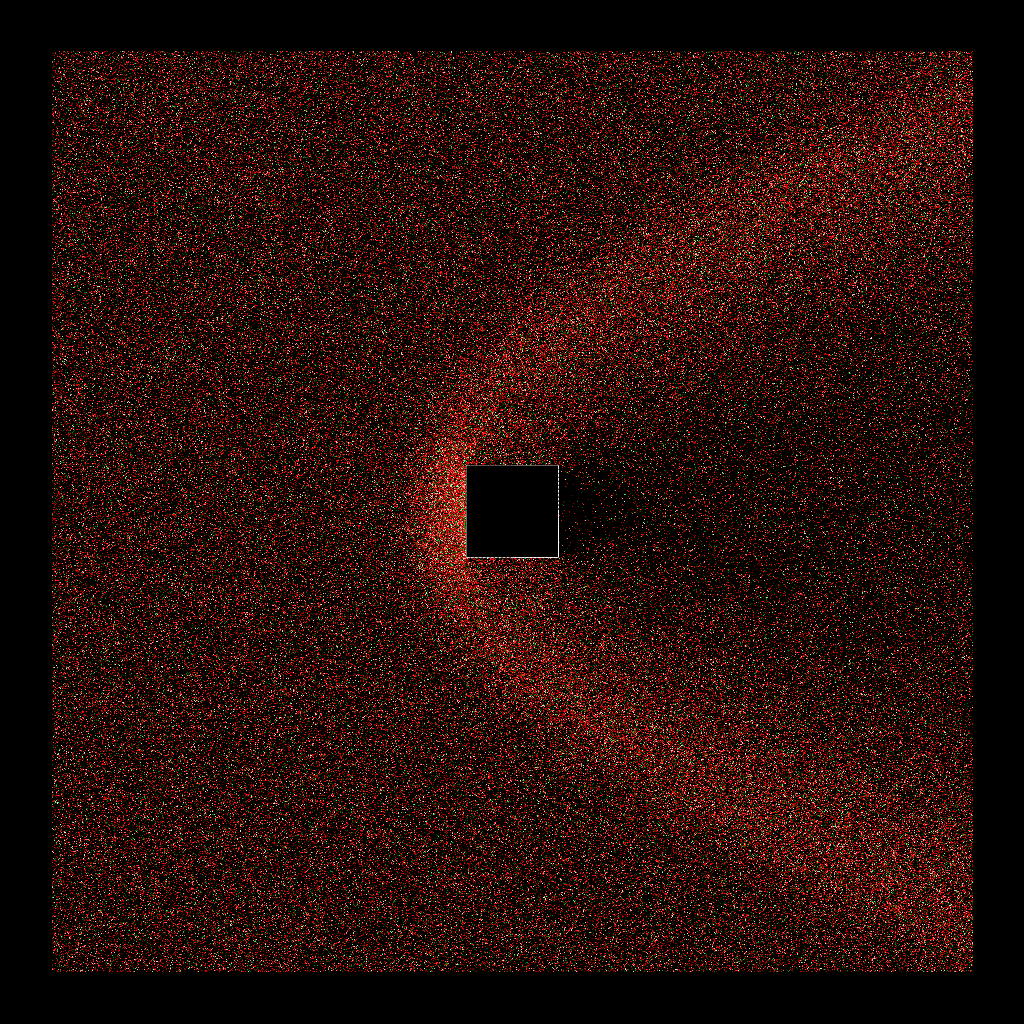
\includegraphics[width=\textwidth]{Images/4. Results/Square Kn/particles/Kn0.1.png}
        \caption{Kn = 0.1}
    \end{subfigure}
    \hfill
    \begin{subfigure}{0.32\textwidth}
        \centering
        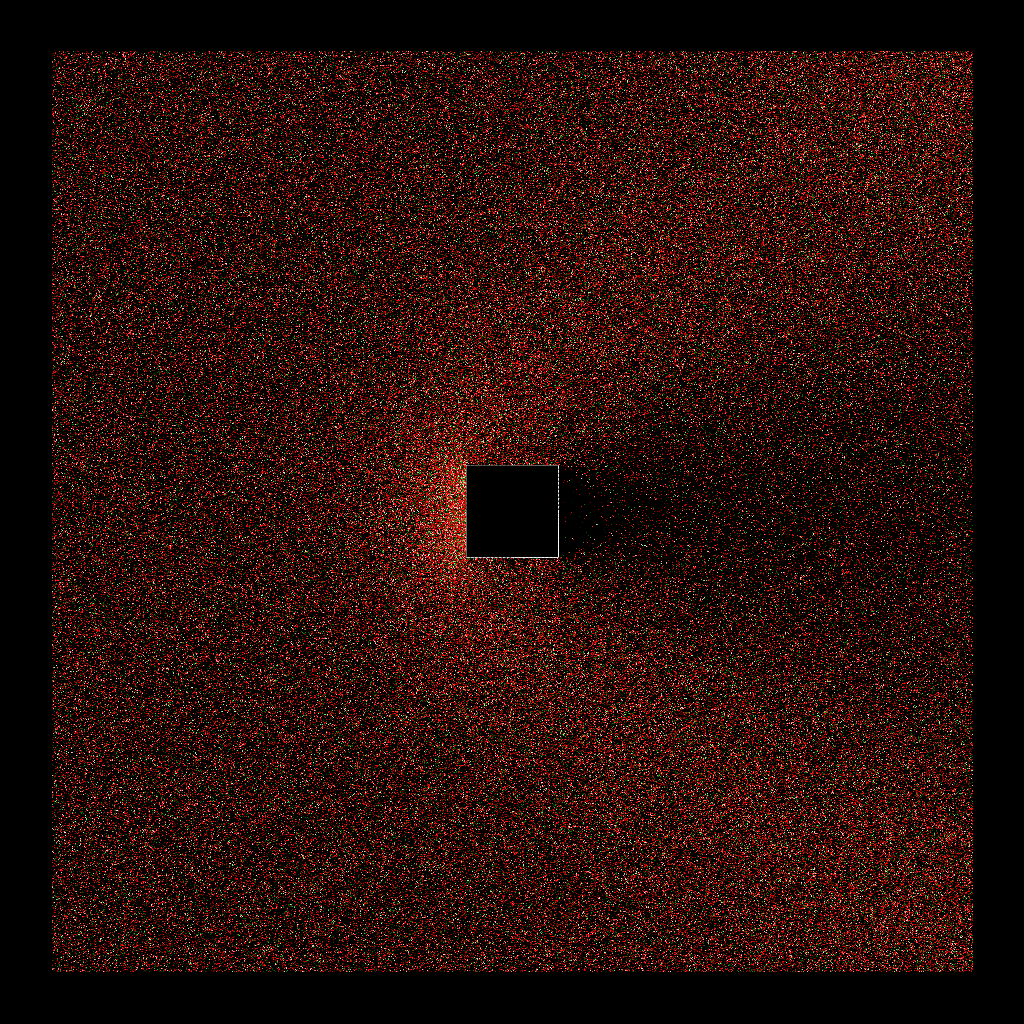
\includegraphics[width=\textwidth]{Images/4. Results/Square Kn/particles/Kn0.5.png}
        \caption{Kn = 0.5}
    \end{subfigure}
    \hfill
    \begin{subfigure}{0.32\textwidth}
        \centering
        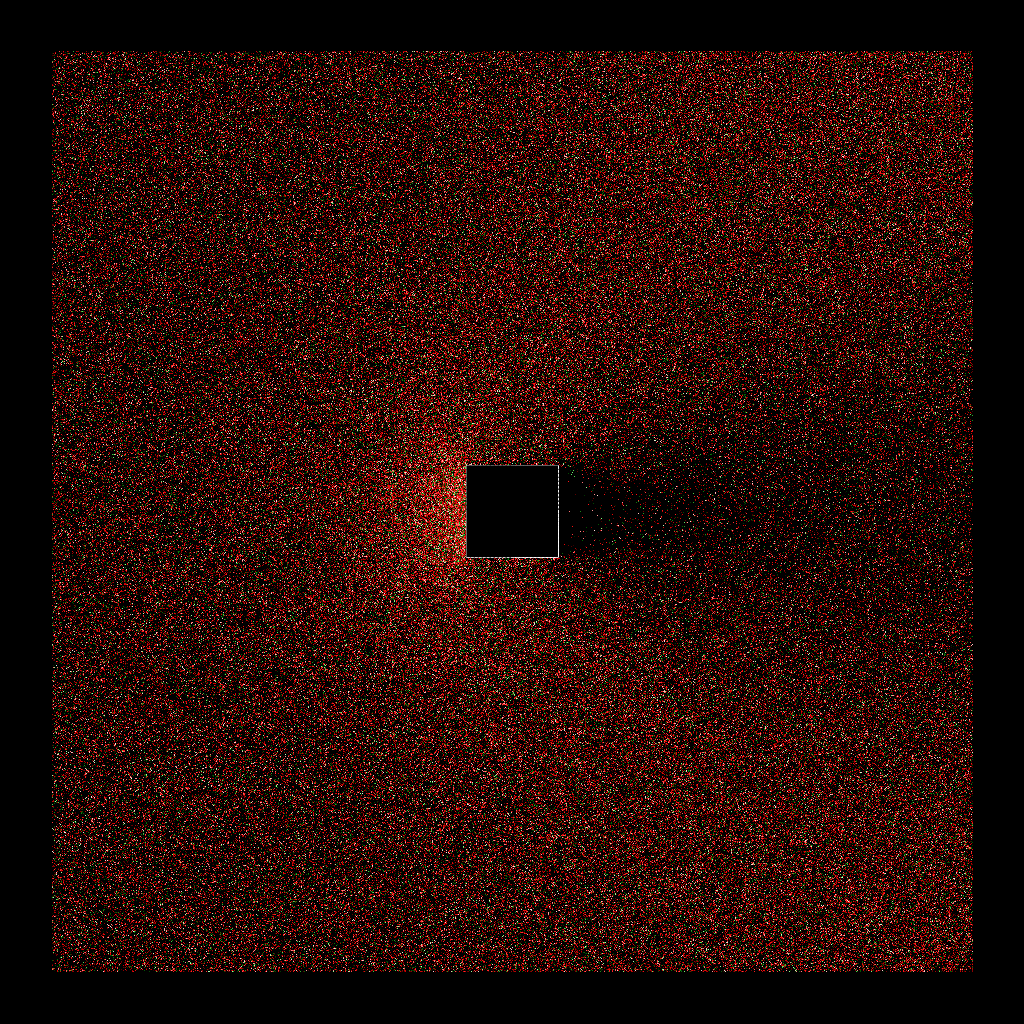
\includegraphics[width=\textwidth]{Images/4. Results/Square Kn/particles/Kn1.png}
        \caption{Kn = 1}
    \end{subfigure}
    
    \vspace{5pt}
    
    \centering
    \begin{subfigure}{0.32\textwidth}
        \centering
        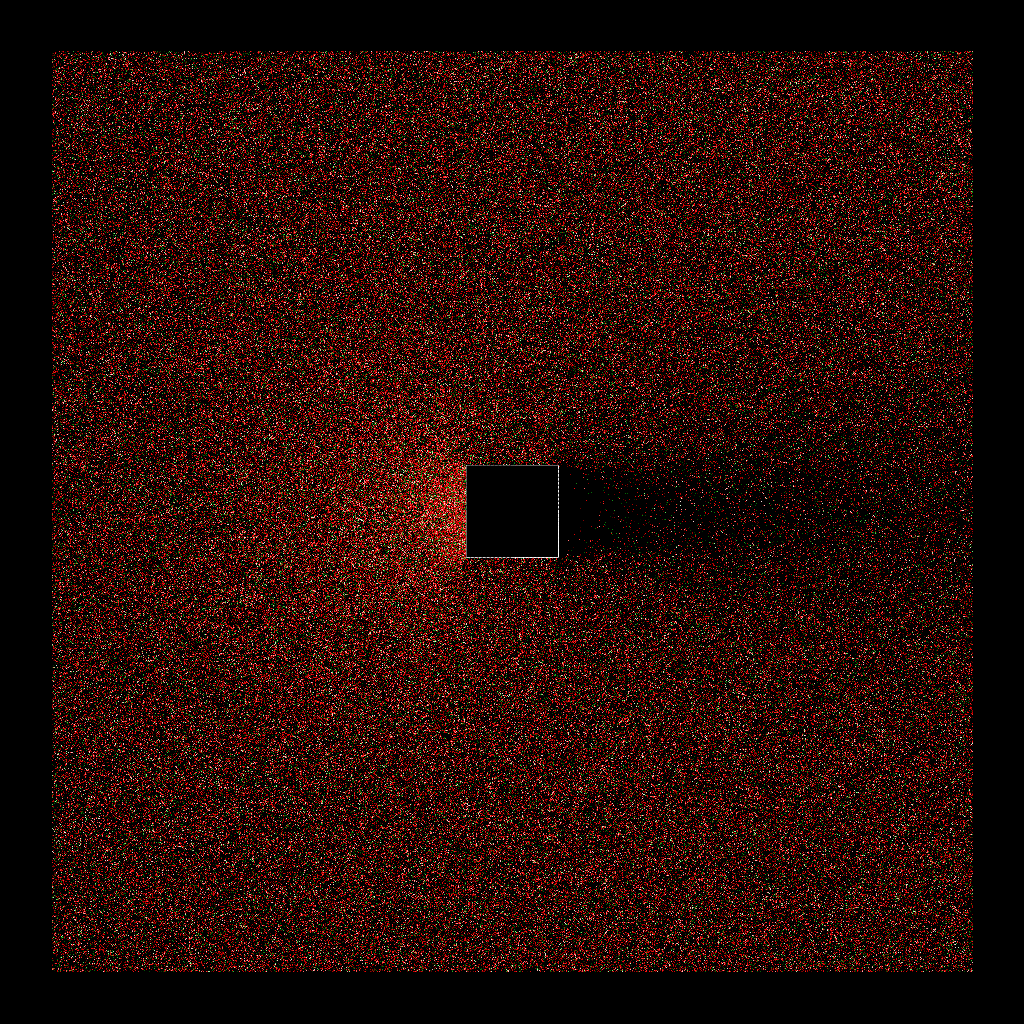
\includegraphics[width=\textwidth]{Images/4. Results/Square Kn/particles/Kn5.png}
        \caption{Kn = 5}
    \end{subfigure}
    \hfill
    \begin{subfigure}{0.32\textwidth}
        \centering
        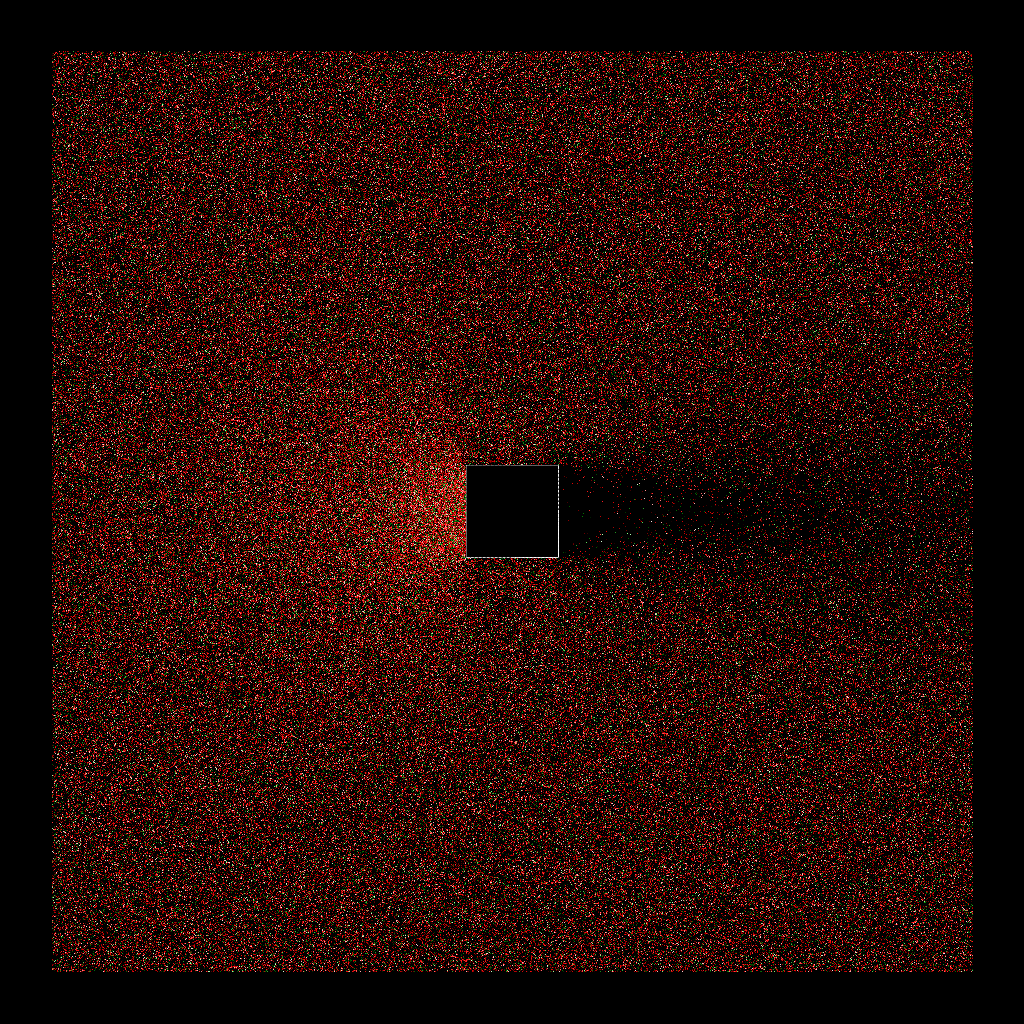
\includegraphics[width=\textwidth]{Images/4. Results/Square Kn/particles/Kn10.png}
        \caption{Kn = 10}
    \end{subfigure}
    \hfill
    \begin{subfigure}{0.32\textwidth}
        \centering
        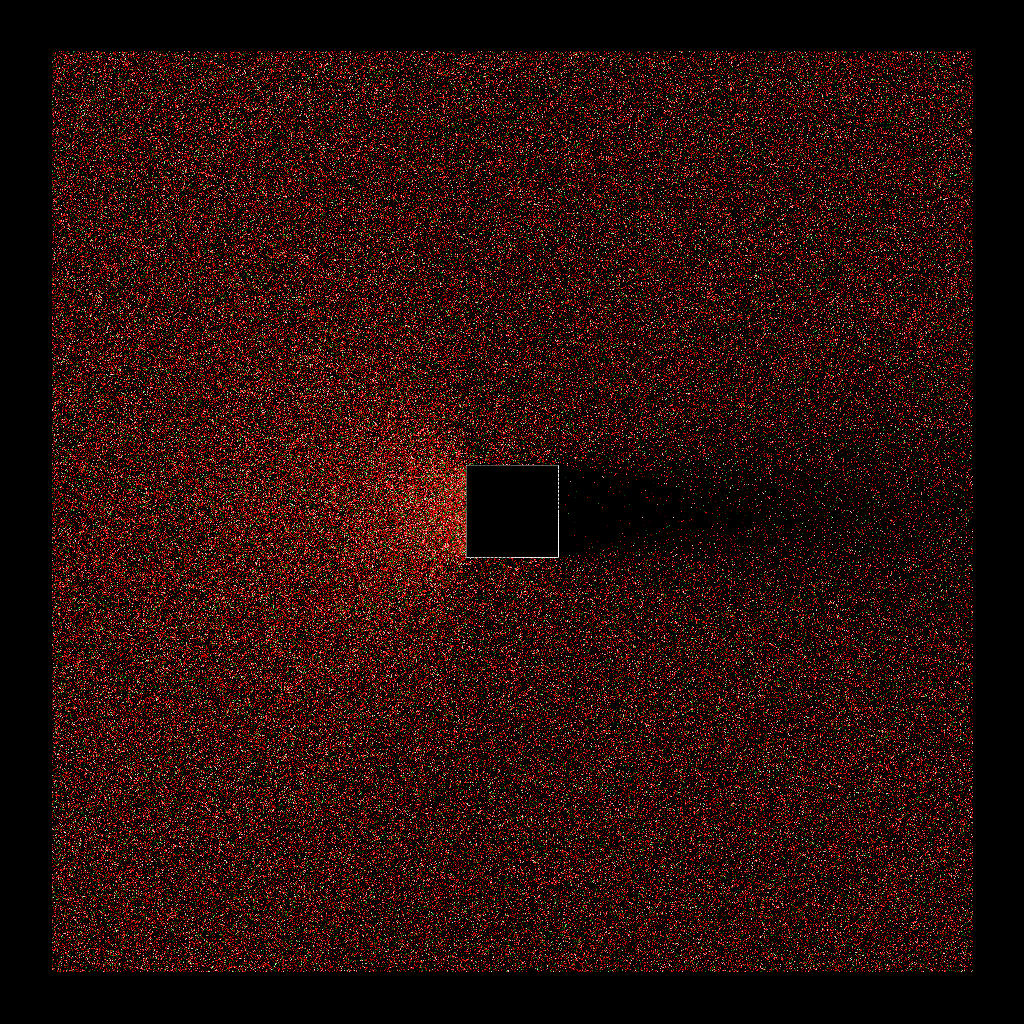
\includegraphics[width=\textwidth]{Images/4. Results/Square Kn/particles/Kn100.png}
        \caption{Kn = 100}
    \end{subfigure}
    \caption{Particle contours around a rounded square for varying Knudsen number.}
    \label{fig:pcontoursquare}
\end{figure}

\begin{figure}
    \centering
    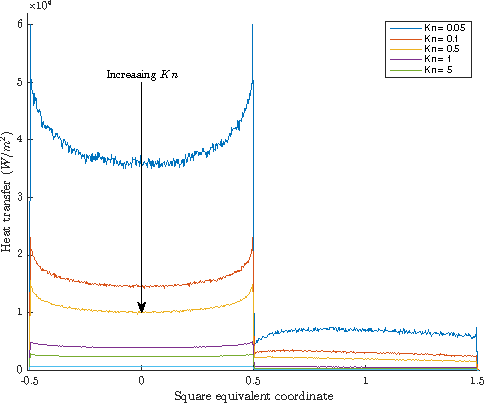
\includegraphics[width=0.52\textwidth]{Images/4. Results/Square Kn/htsec.pdf}
    \caption{Distribution of heat transfer along the square contour for varying values of Knudsen number}
    \label{fig:squarehtsec}
\end{figure}

\begin{figure}
    \centering
    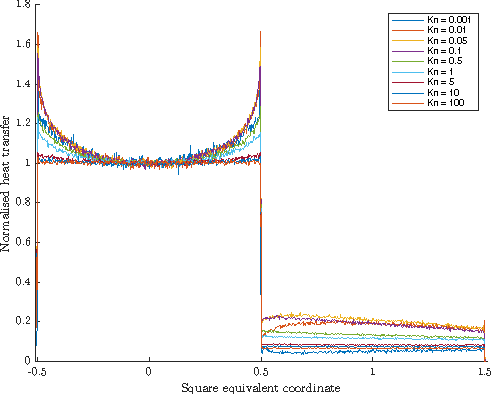
\includegraphics[width=0.52\textwidth]{Images/4. Results/Square Kn/nhtsec.pdf}
    \caption{Distribution of normalised heat transfer along the square contour for varying values of Knudsen number}
    \label{fig:squarenhtsec}
\end{figure}

\begin{figure}
    \centering
    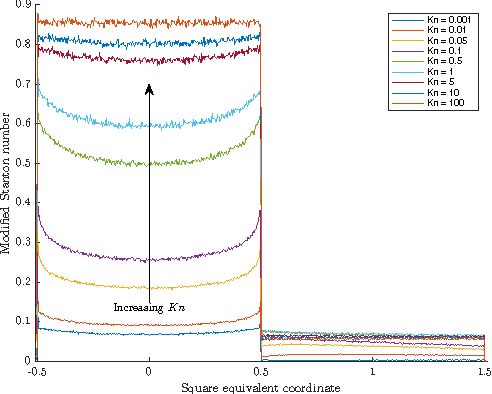
\includegraphics[width=0.52\textwidth]{Images/4. Results/Square Kn/stsec.pdf}
    \caption{Distribution of modified Stanton number along the square contour for varying values of Knudsen number}
    \label{fig:squarestsec}
\end{figure}

\autoref{fig:squarehtsec} shows the distribution of heat transfer along the square contour for varying values of Knudsen number. A very significant reduction in heat transfer is observed with increased Knudsen number. This is probably caused by the decrease in density of the flow.

\autoref{fig:squarenhtsec} shows the heat transfer contours normalised by stagnation point heating. Peaks in heat transfer similar to those noted in \cite{rees} can be seen at the corners of the square for low Knudsen numbers. These peaks, however, disappear as the Knudsen number is increased. This is probably due to the change in flow physics explained above: as the flow is not forced to turn around the corner, its velocity does not increase and as a result the heat transfer profile flattens out.

\autoref{fig:squarestsec} shows the distribution of modified Stanton number along the square contour for varying of Knudsen numbers. The significant increase in Stanton number seen with increasing Knudsen number can again be probably explained by the change in flow physics with Knudsen number: as $Kn$ is increased, the high density region between the shock and the cube's stagnation surface gradually dissipates, disappearing completely at very high Knudsen numbers. Consequently, the particles that collide with the cube's surface lose less energy, as they don't undergo collisions with molecules in the high-density region. This results in an higher energy transfer during the subsequent impact with the cube, leading to an increase in Stanton number.


Similar flow physics and heating trends were observed for a circle geometry. They can be seen in \autoref{fig:vcontourcircle} and \autoref{fig:heatcontourcircle}. 

\begin{figure}
    \centering
    \begin{subfigure}{0.32\textwidth}
        \centering
        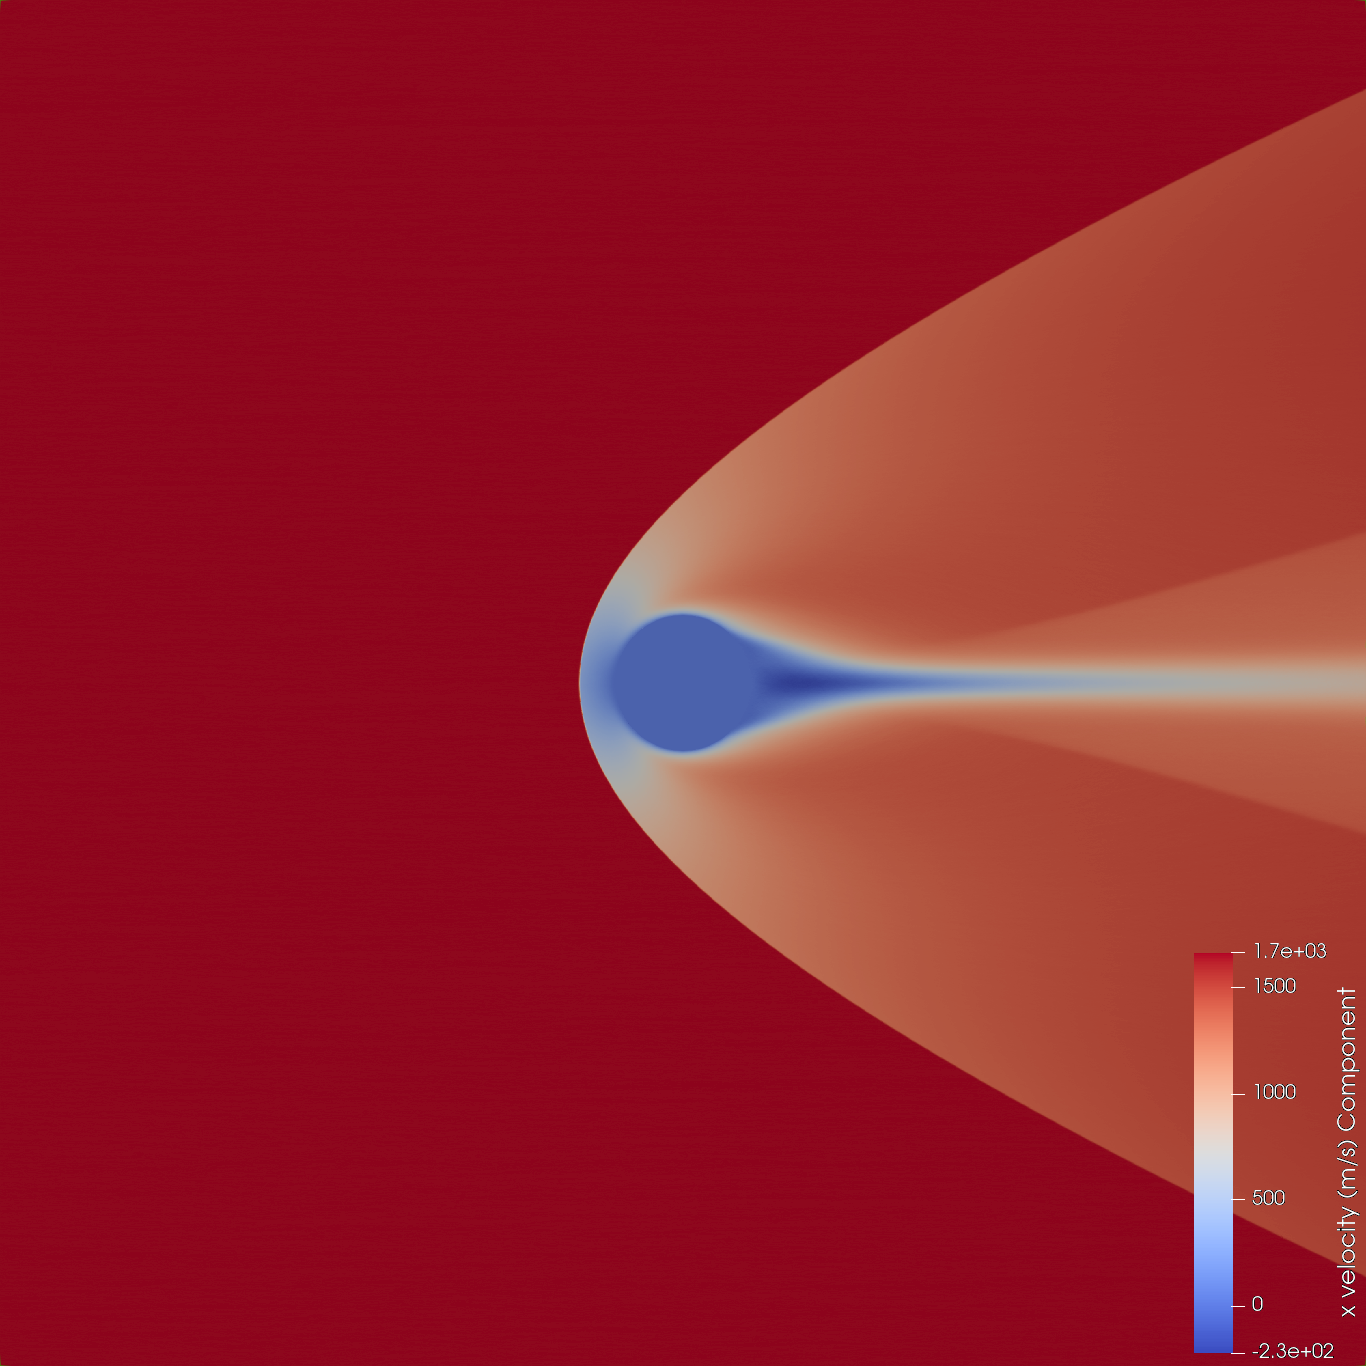
\includegraphics[width=\textwidth]{Images/4. Results/Circle Kn/pv/Kn0.001.png}
        \caption{Kn = 0.001}
    \end{subfigure}
    \hfill
    \begin{subfigure}{0.32\textwidth}
        \centering
        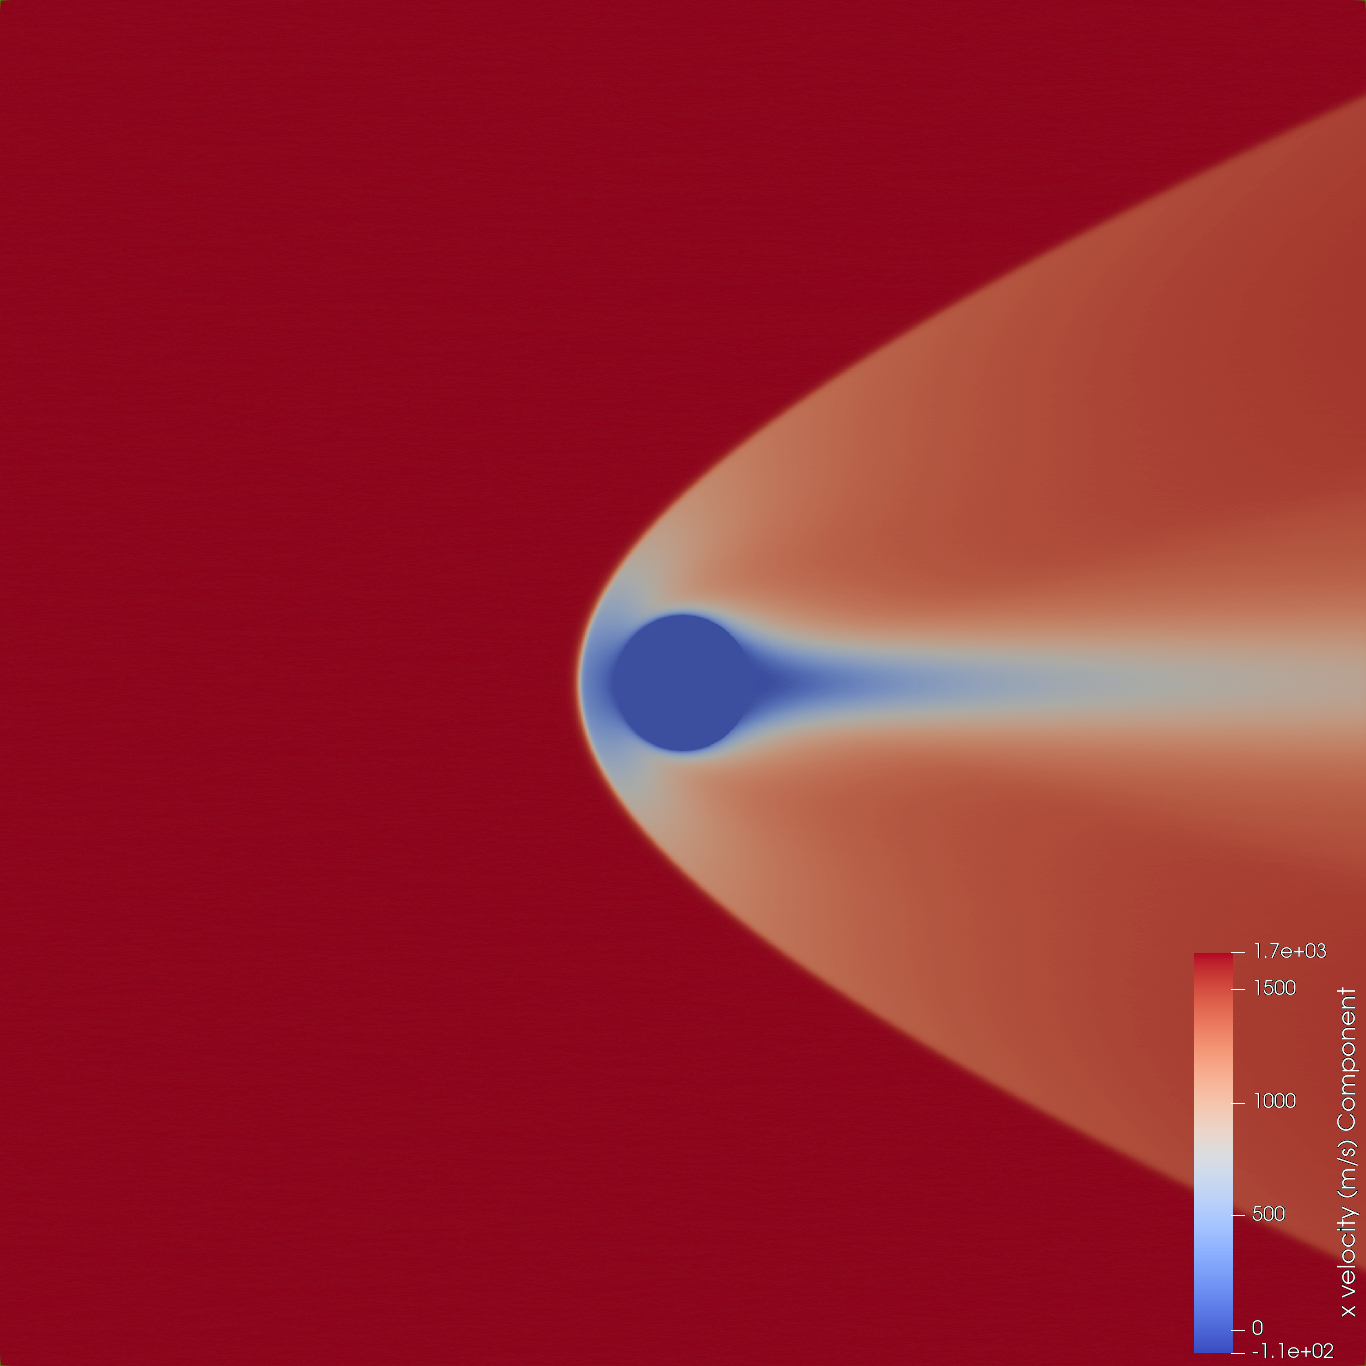
\includegraphics[width=\textwidth]{Images/4. Results/Circle Kn/pv/Kn0.01.png}
        \caption{Kn = 0.01}
    \end{subfigure}
    \hfill
    \begin{subfigure}{0.32\textwidth}
        \centering
        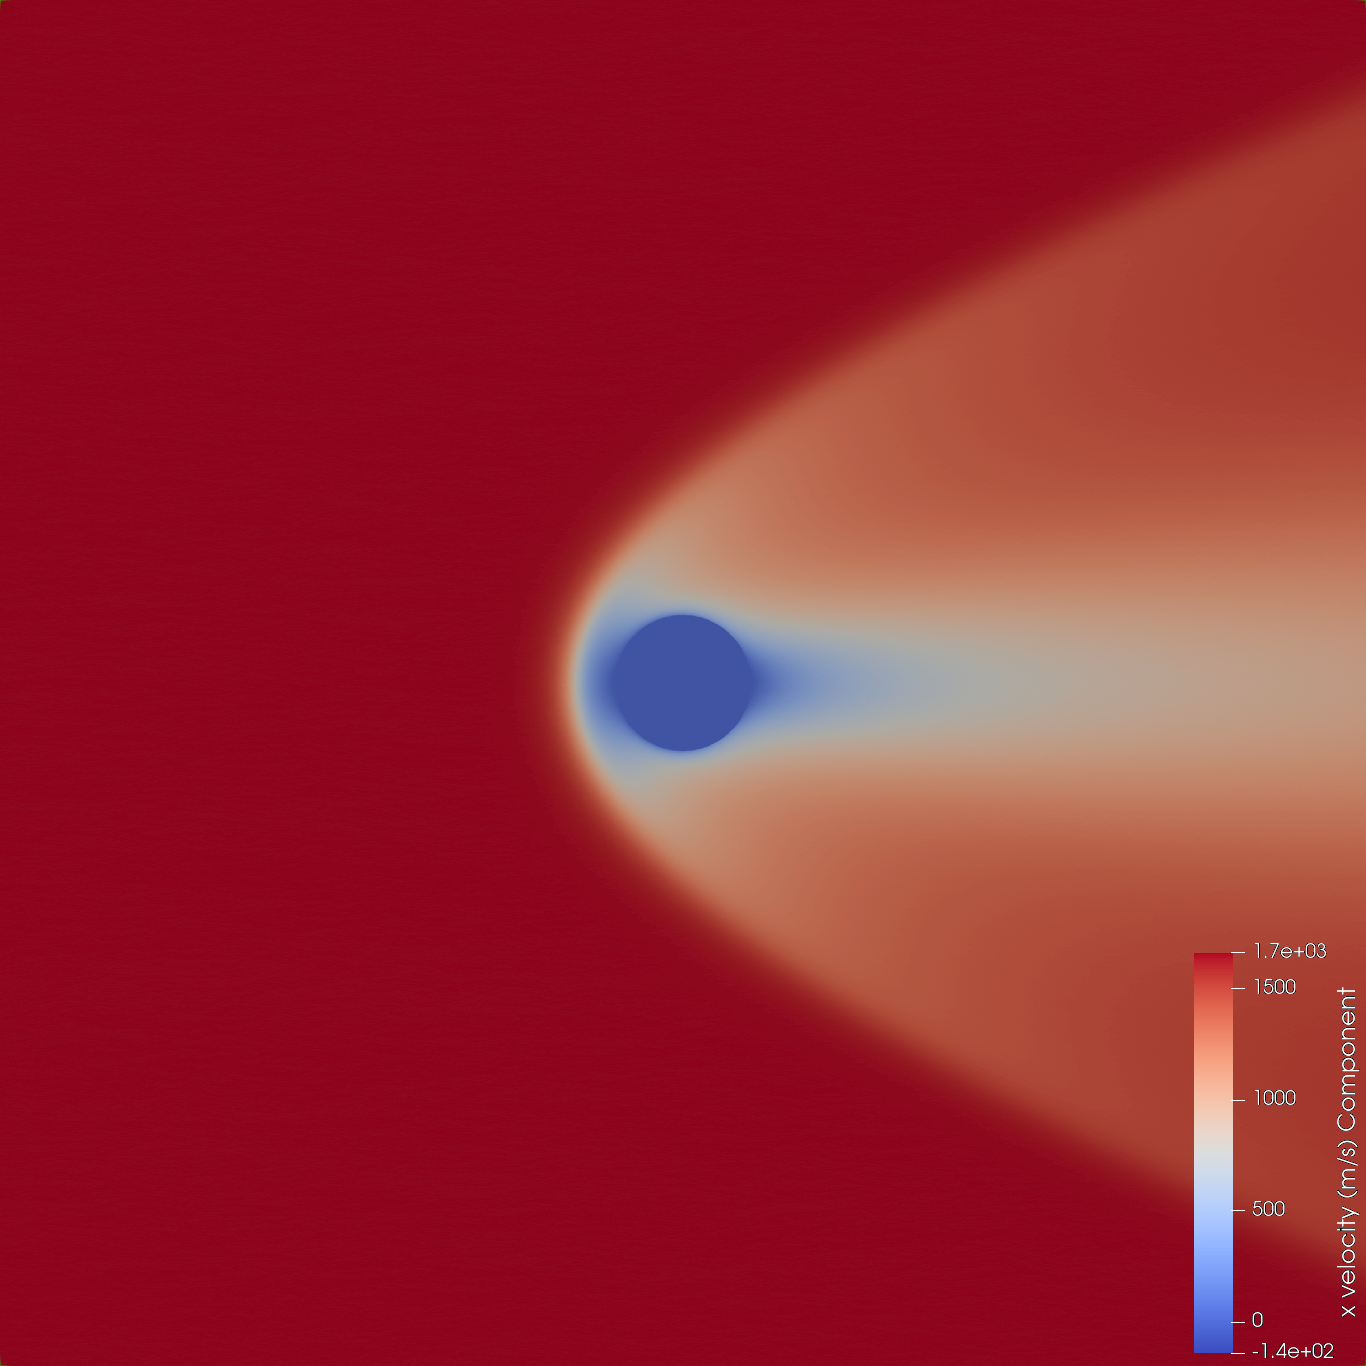
\includegraphics[width=\textwidth]{Images/4. Results/Circle Kn/pv/Kn0.05.png}
        \caption{Kn = 0.05}
    \end{subfigure}
    
    \vspace{5pt}
    
    \centering
    \begin{subfigure}{0.32\textwidth}
        \centering
        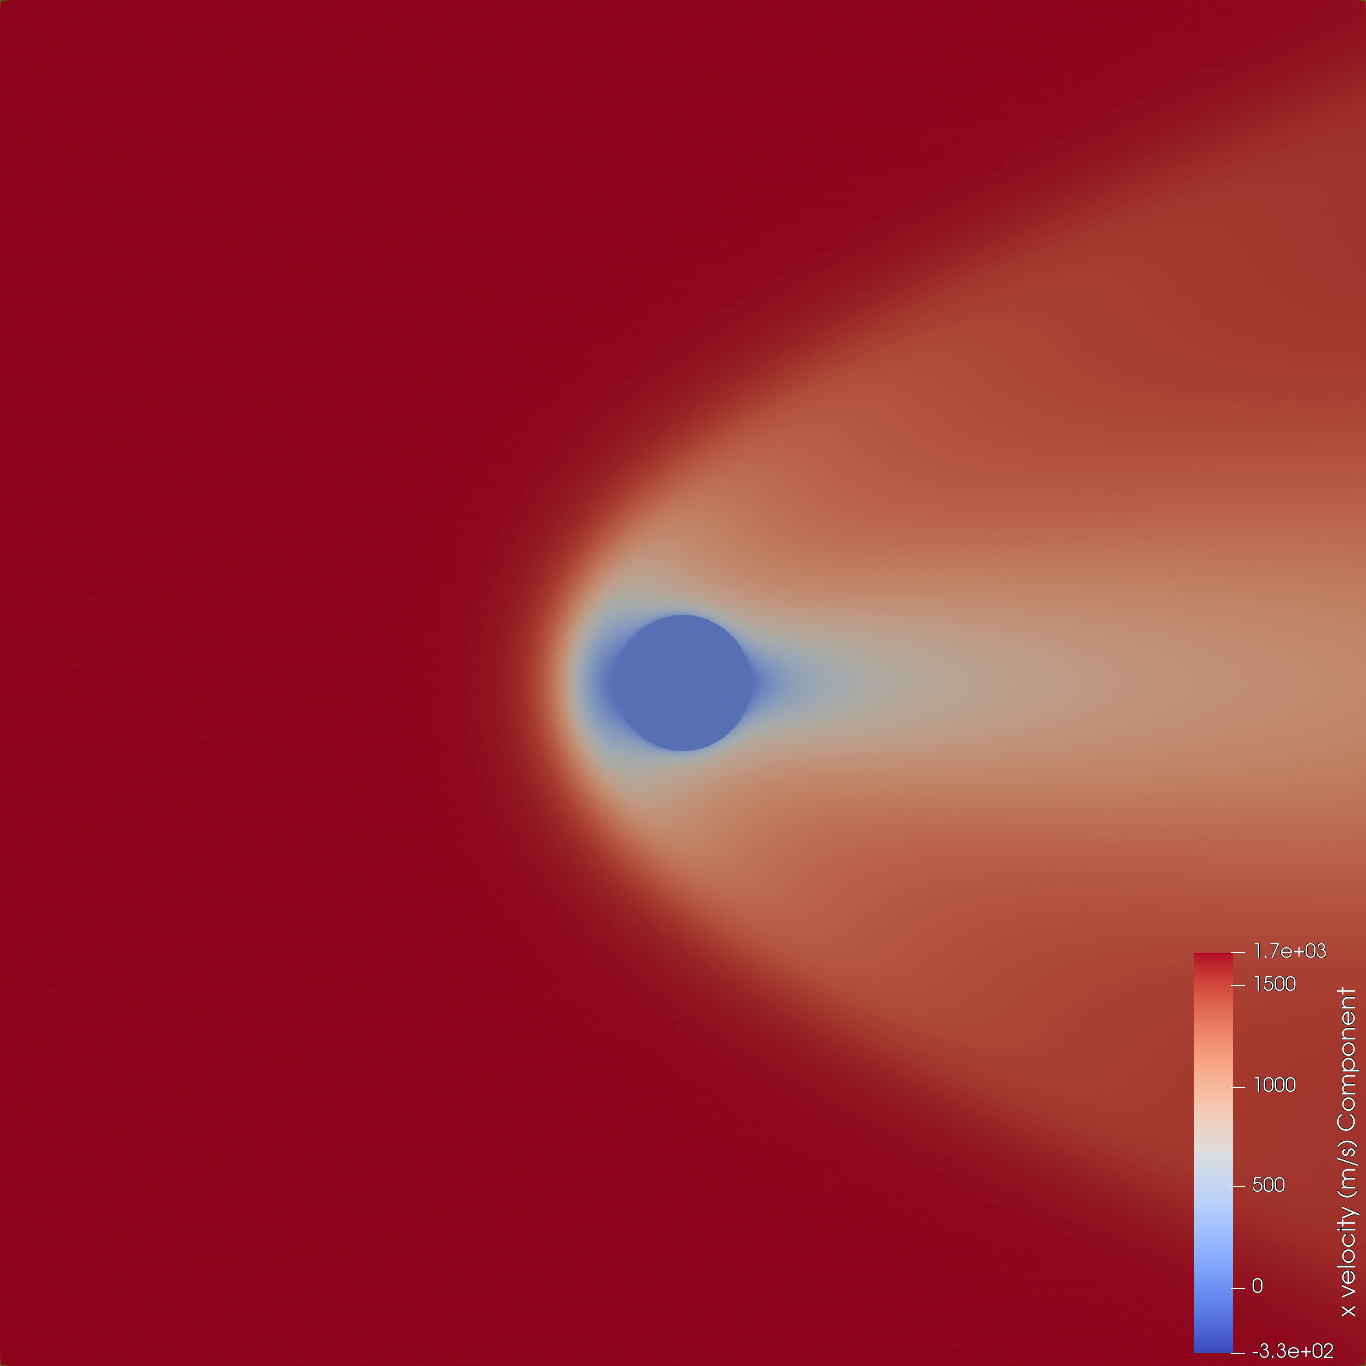
\includegraphics[width=\textwidth]{Images/4. Results/Circle Kn/pv/Kn0.1.png}
        \caption{Kn = 0.1}
    \end{subfigure}
    \hfill
    \begin{subfigure}{0.32\textwidth}
        \centering
        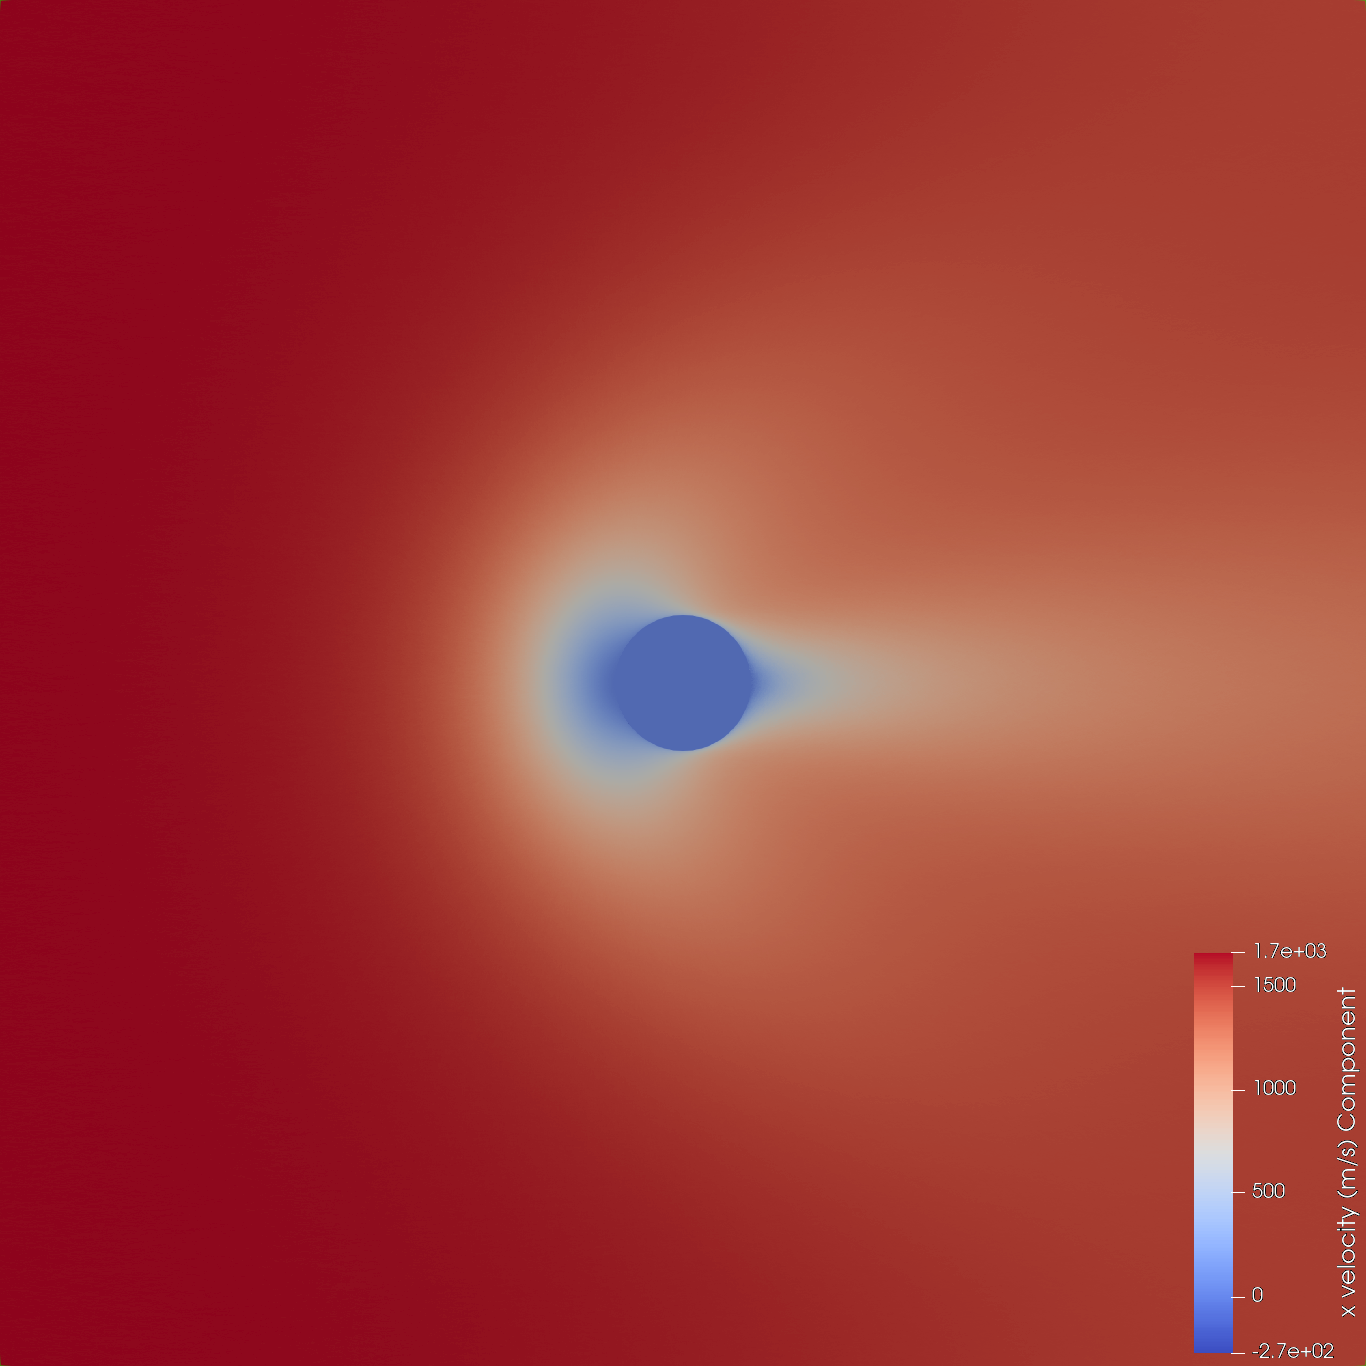
\includegraphics[width=\textwidth]{Images/4. Results/Circle Kn/pv/Kn0.5.png}
        \caption{Kn = 0.5}
    \end{subfigure}
    \hfill
    \begin{subfigure}{0.32\textwidth}
        \centering
        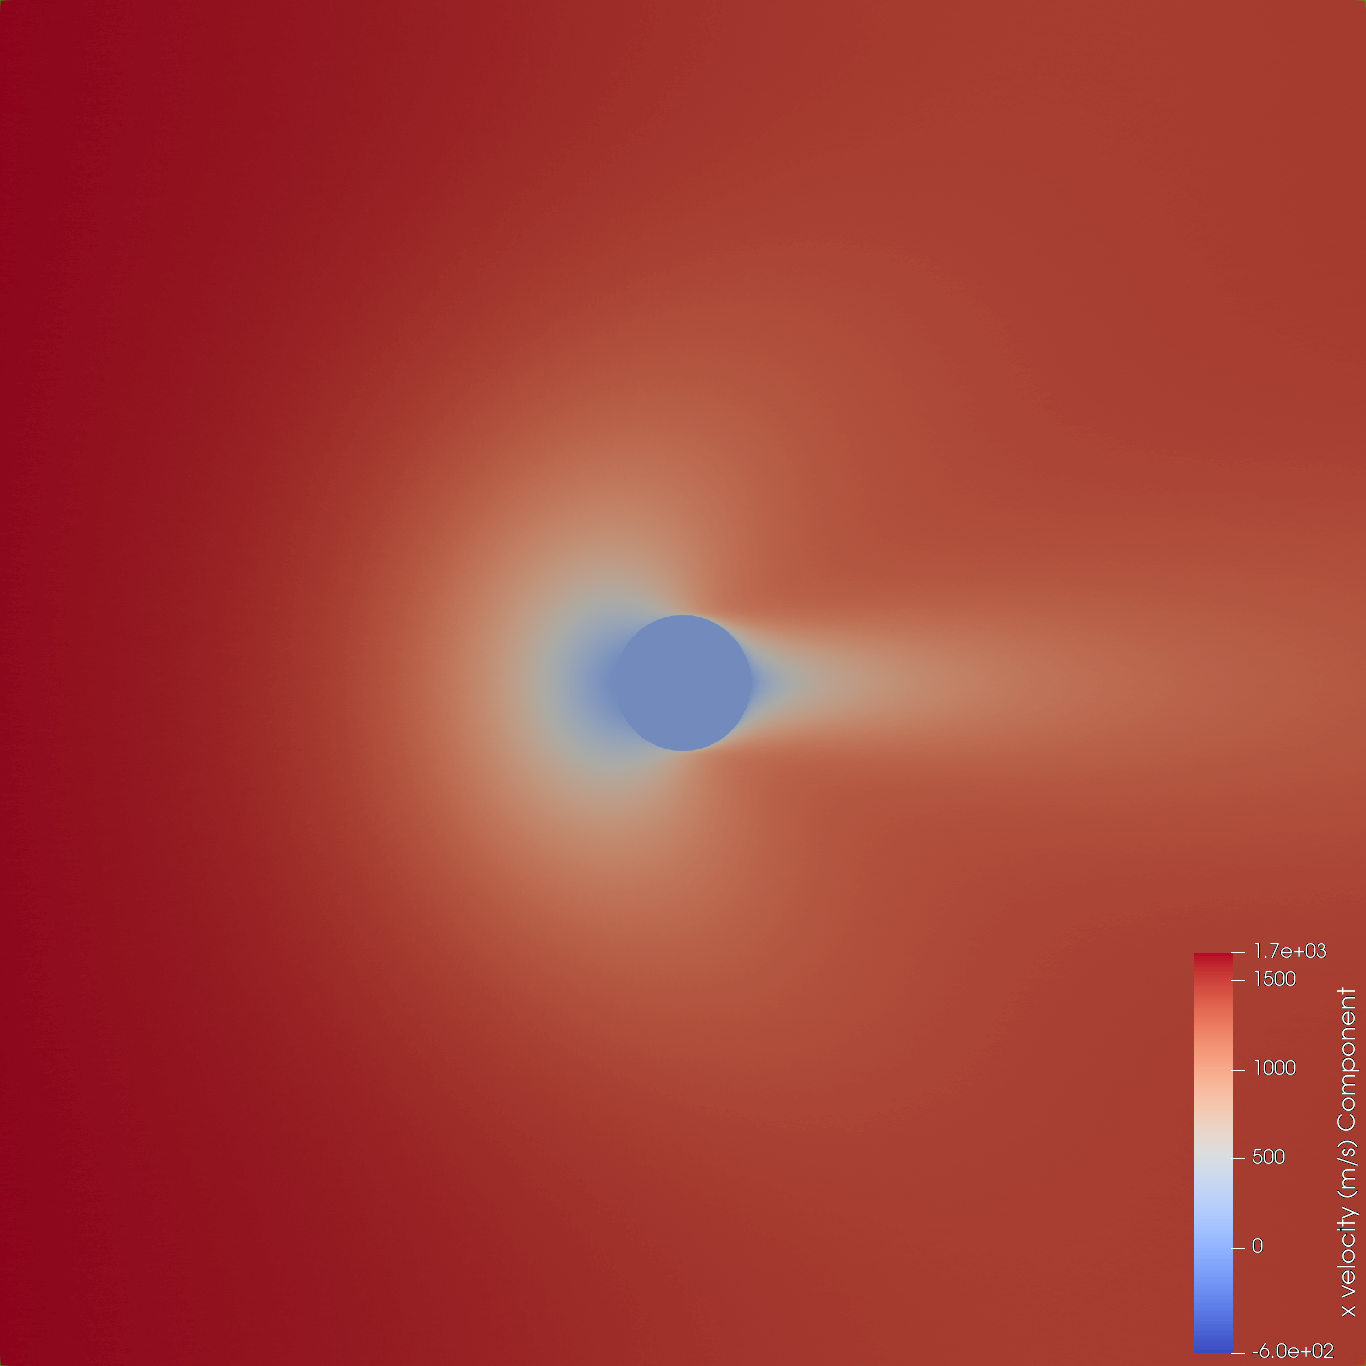
\includegraphics[width=\textwidth]{Images/4. Results/Circle Kn/pv/Kn1.png}
        \caption{Kn = 1}
    \end{subfigure}
    
    \vspace{5pt}
    
    \centering
    \begin{subfigure}{0.32\textwidth}
        \centering
        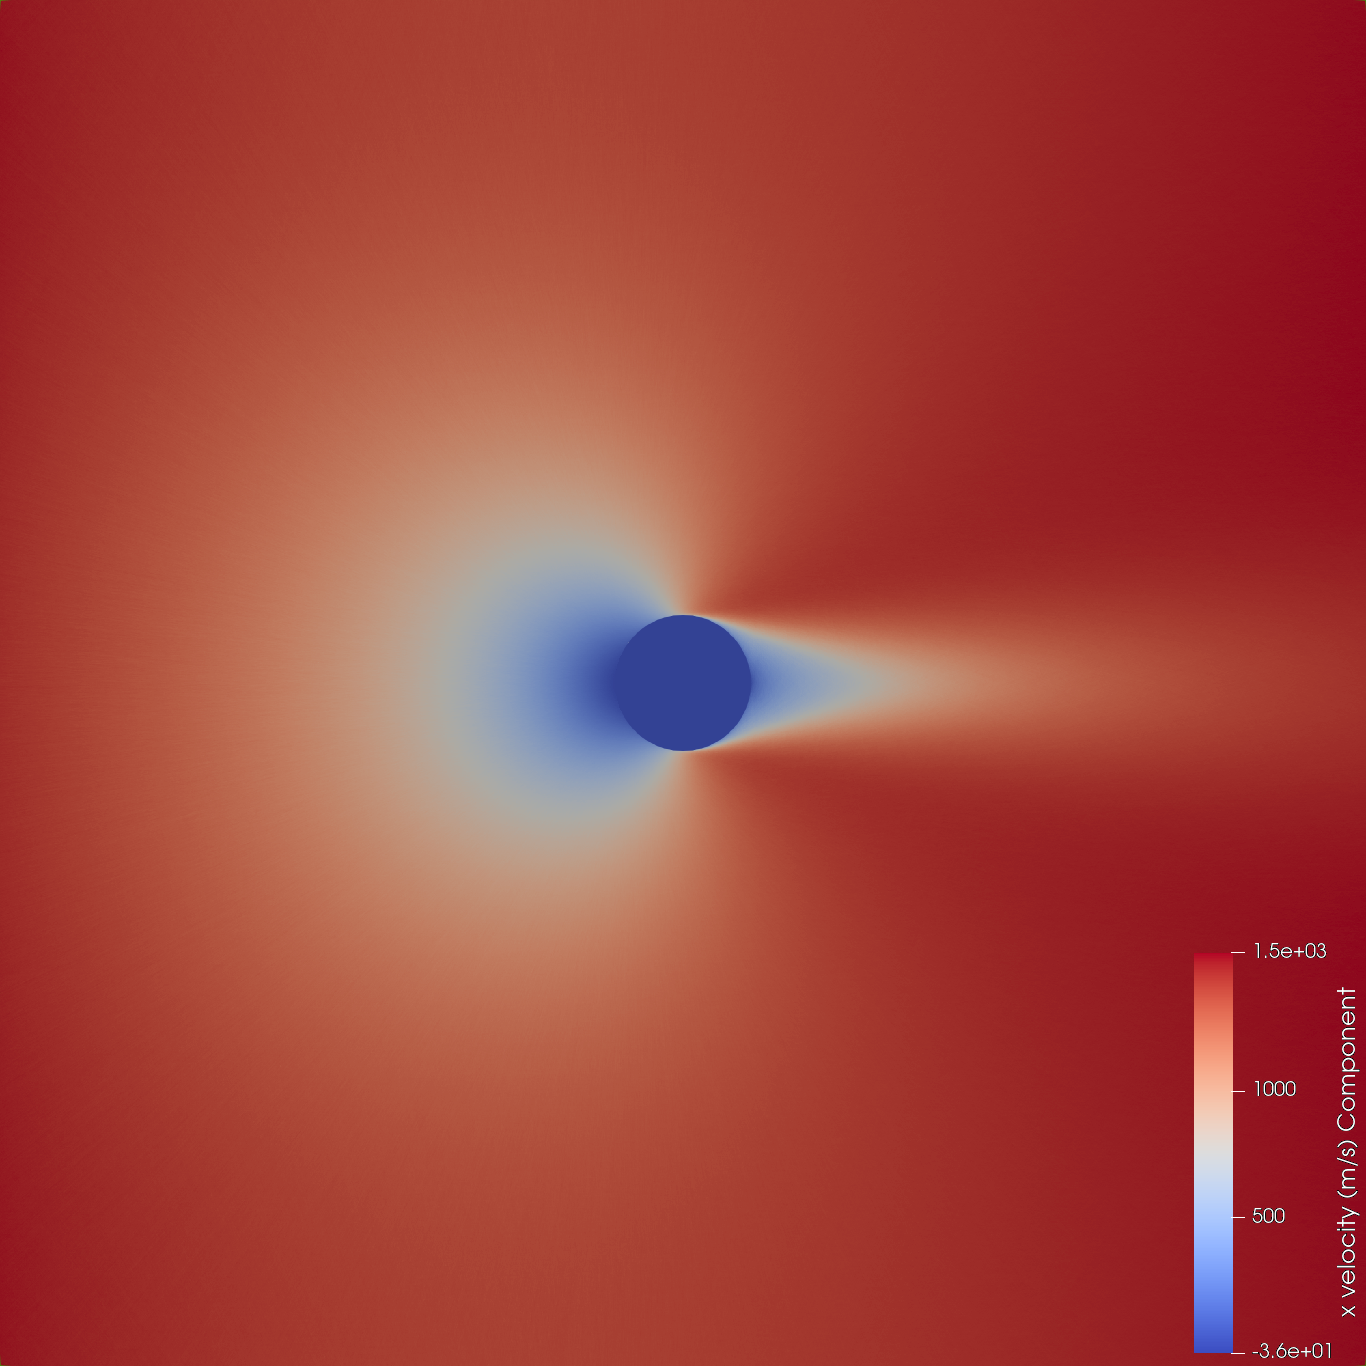
\includegraphics[width=\textwidth]{Images/4. Results/Circle Kn/pv/Kn5.png}
        \caption{Kn = 5}
    \end{subfigure}
    \hfill
    \begin{subfigure}{0.32\textwidth}
        \centering
        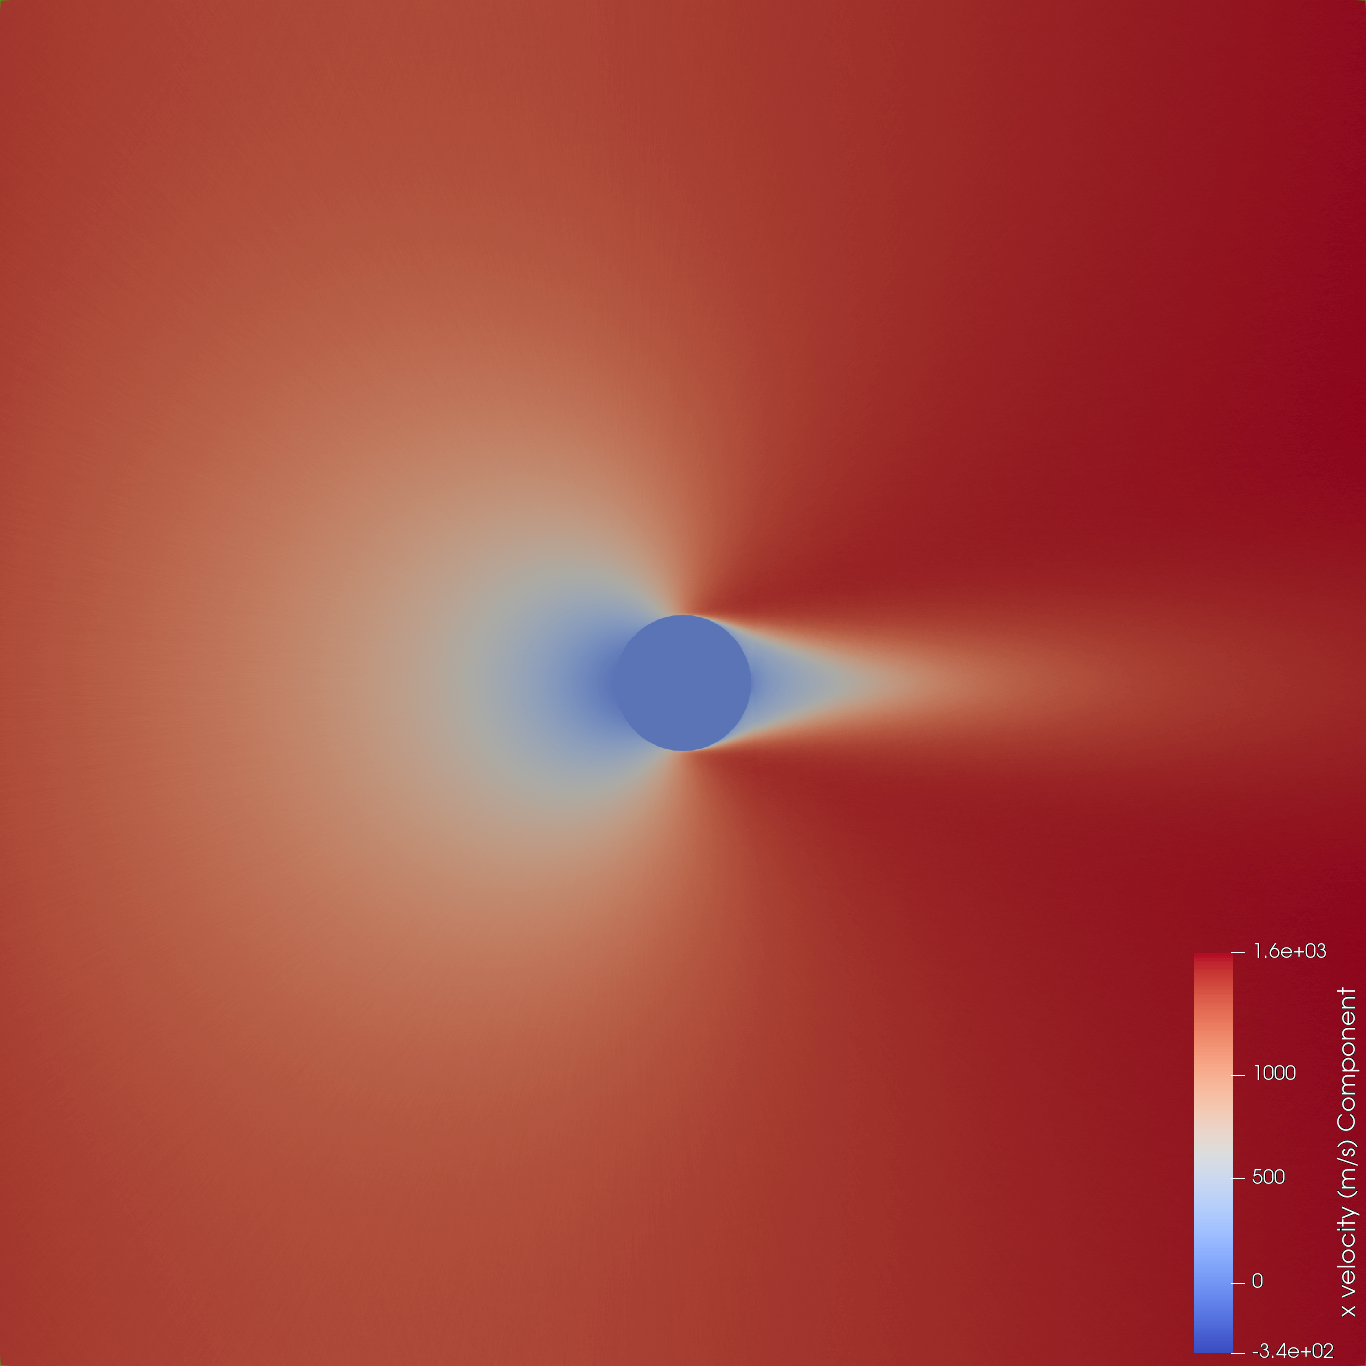
\includegraphics[width=\textwidth]{Images/4. Results/Circle Kn/pv/Kn10.png}
        \caption{Kn = 10}
    \end{subfigure}
    \hfill
    \begin{subfigure}{0.32\textwidth}
        \centering
        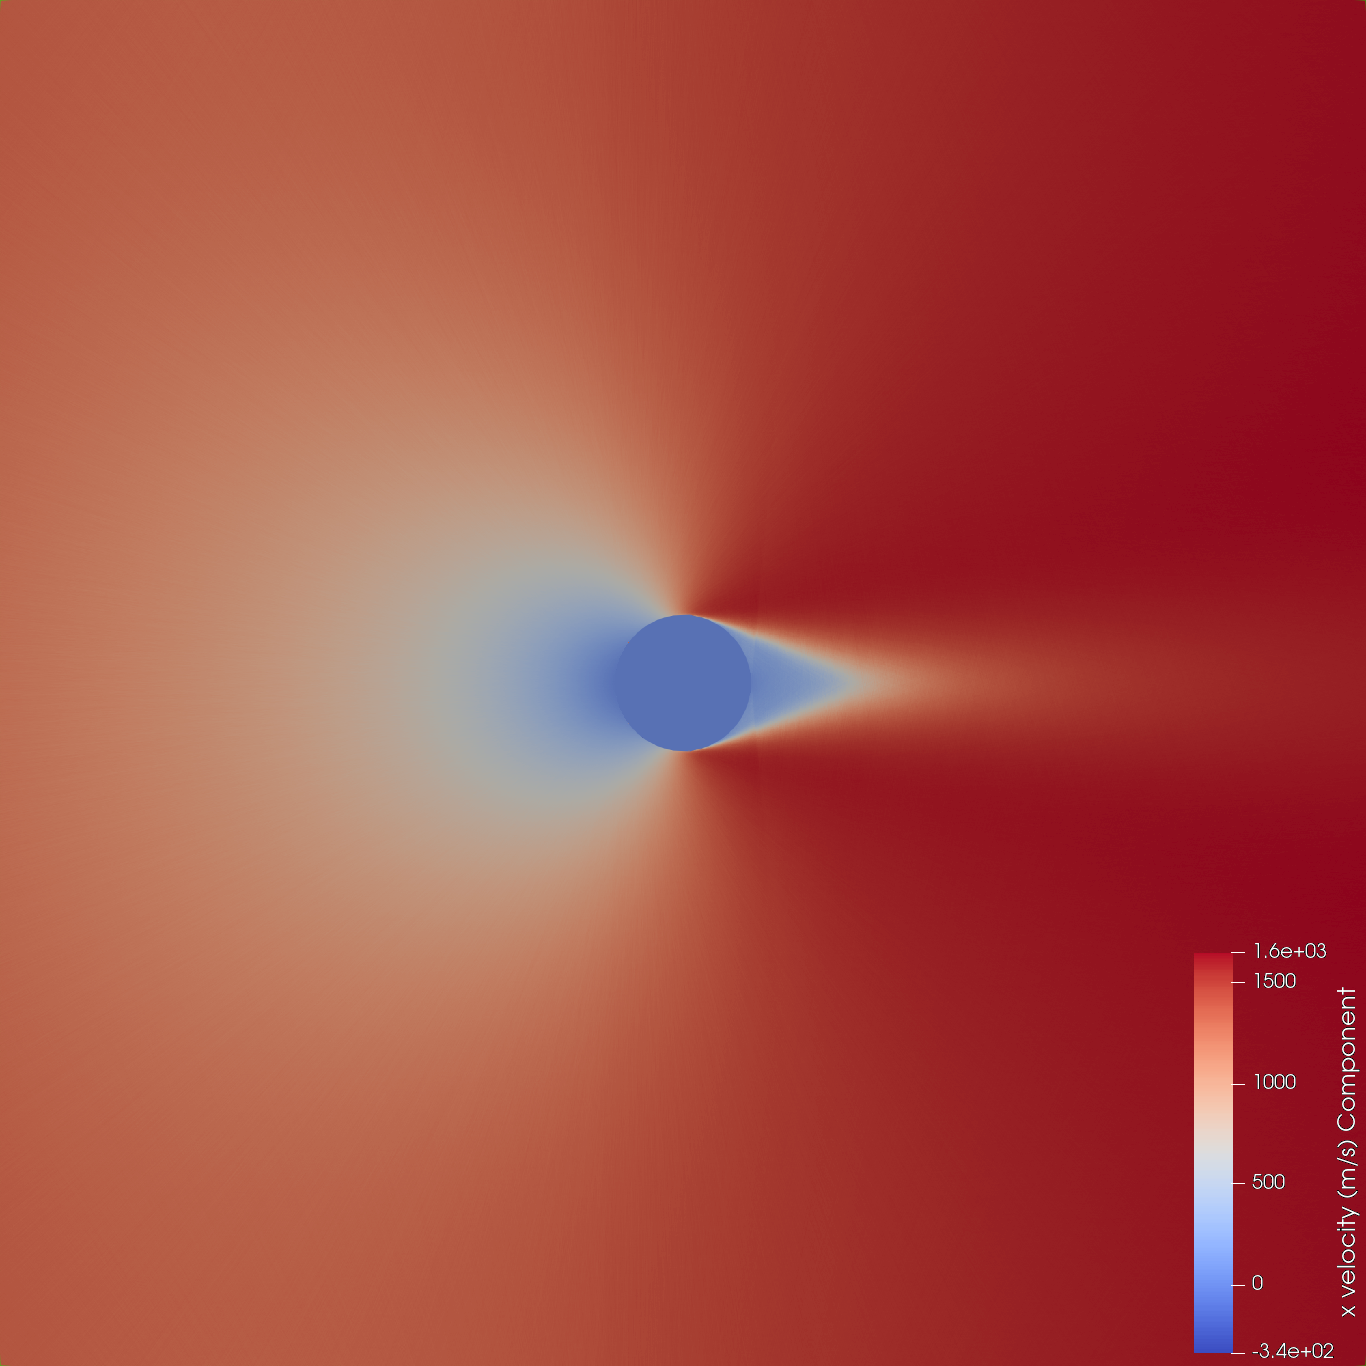
\includegraphics[width=\textwidth]{Images/4. Results/Circle Kn/pv/Kn100.png}
        \caption{Kn = 100}
    \end{subfigure}
    \caption{Velocity contours around a circle for varying Knudsen number.}
    \label{fig:vcontourcircle}
\end{figure}

\begin{figure}
    \centering
    \begin{subfigure}{0.49\textwidth}
        \centering
        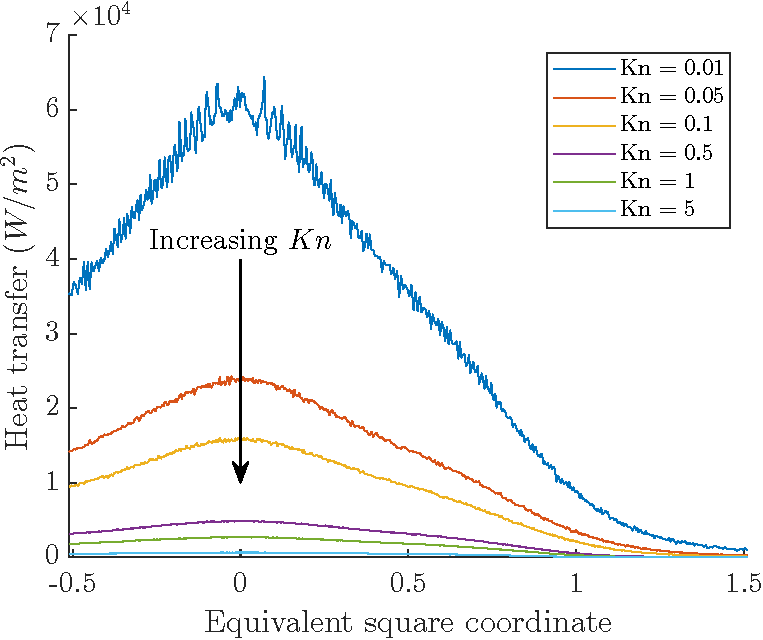
\includegraphics[width=\textwidth]{Images/4. Results/Circle Kn/htsec.pdf}
    \end{subfigure}
    \hfill
    \begin{subfigure}{0.49\textwidth}
        \centering
        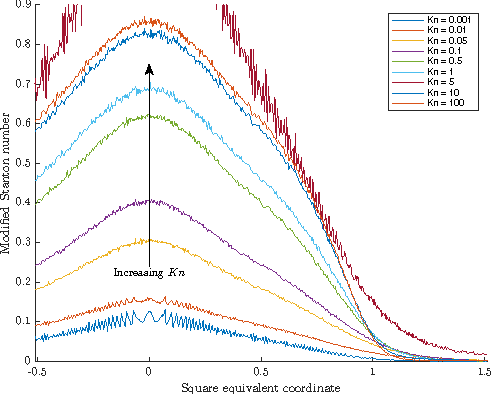
\includegraphics[width=\textwidth]{Images/4. Results/Circle Kn/stsec.pdf}
    \end{subfigure}
    \caption{Heating (left) and stagnation Stanton number (right) distribution around a circle for varying Knudsen number.}
    \label{fig:heatcontourcircle}
\end{figure}

The variation in stagnation point Stanton number observed in \autoref{fig:squarestsec} and \autoref{fig:heatcontourcircle} have been plotted respectively in \autoref{fig:stantonsquare} and \autoref{fig:stantoncircle}, with respect to the global Knudsen number, calculated based on the square side length. The observed pattern is partly matched by the one observed in literature for spheres \cite{riabov}, shown in \autoref{fig:riabov}. The behaviour for Knudsen numbers below 0.01 could not be compared, due to lack of experimental data.

\begin{figure}
    \centering
    \begin{subfigure}{0.49\textwidth}
        \centering
        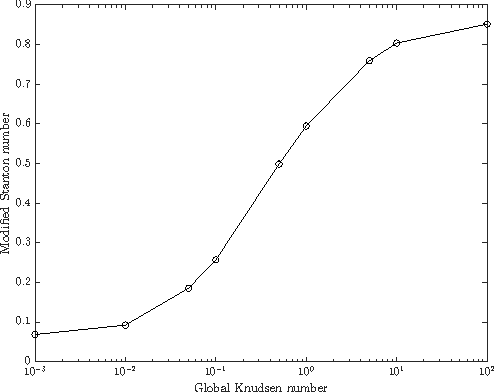
\includegraphics[width=\textwidth]{Images/4. Results/Square Kn/stkn.pdf}
        \caption{Square}
        \label{fig:stantonsquare}
    \end{subfigure}
    \hfill
    \begin{subfigure}{0.49\textwidth}
        \centering
        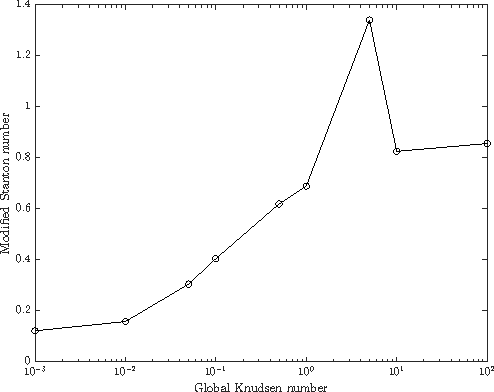
\includegraphics[width=\textwidth]{Images/4. Results/Circle Kn/stkn.pdf}
        \caption{Circle}
        \label{fig:stantoncircle}
    \end{subfigure}
    \caption{Stanton number vs global Knudsen number for a rounded square (a) and circle (b).}
    \label{fig:stanton}
\end{figure}

\begin{figure}
    \centering
    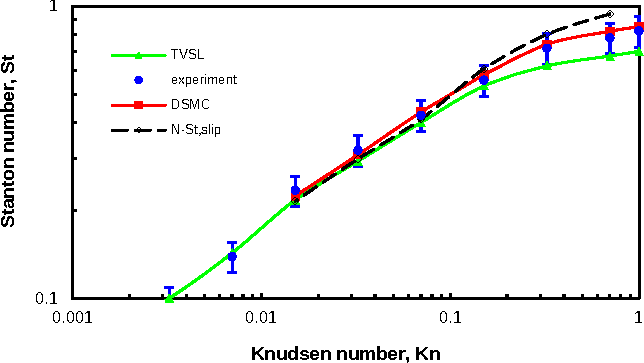
\includegraphics{Images/4. Results/riabov.pdf}
    \caption{Stanton number vs global Knudsen number from literature \cite{riabov}.}
    \label{fig:riabov}
\end{figure}

The variation in ratio between the peak and stagnation point Stanton number has been calculated and plotted against the local Knudsen number at the square corner. It can be seen in \autoref{fig:ratiokn}. The trend shown by it mostly appears as it would have been expected based on the intuition gained from the velocity contours above. The point at $Kn = 0.1$ is however, shows a slightly lower value from the peak at $Kn = 1$. The reason for this dip is not entirely clear, and will be discussed more in depth in \autoref{subsection:comparison}.

\begin{figure}
    \centering
    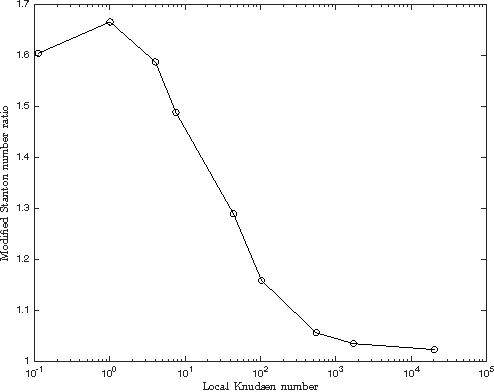
\includegraphics[width=0.6\textwidth]{Images/4. Results/Square Kn/stratiolocalkn.pdf}
    \caption{Stanton number ratio vs local Knudsen number for the varying global Knudsen number test case.}
    \label{fig:ratiokn}
\end{figure}

\subsection{Variation of edge radius results}

\autoref{fig:radiushtsec} shows the distribution of heat transfer around the geometry for varying values of edge radius. Note that, for clarity reasons, not all of the simulation cases have been included. It is possible to note that as the corner radius is increased, the reduction in heat transfer past the corner peak becomes more gradual, and the two peaks at the square edged coalesce into one. Because of the same effect, the heat transfer at the stagnation point gradually increases.

Comparing \autoref{fig:radiushtsec} to \autoref{fig:squarehtsec}, reveals that the order of magnitude reduction in heat transfer has disappeared, as the global Knudsen number (and thus the density) has been kept constant.

\begin{figure}
    \centering
    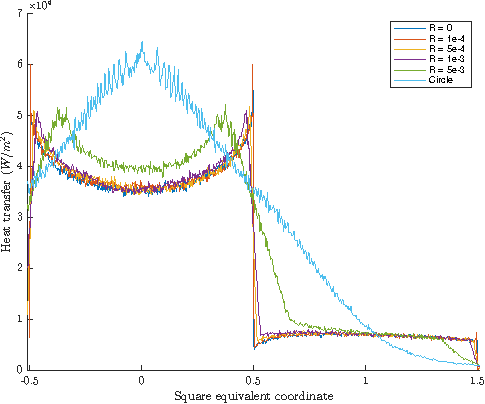
\includegraphics[width=0.52\textwidth]{Images/4. Results/Radius/htsec.pdf}
    \caption{Distribution of heat transfer along the square contour for varying values edge radius.}
    \label{fig:radiushtsec}
\end{figure}

\begin{figure}
    \centering
    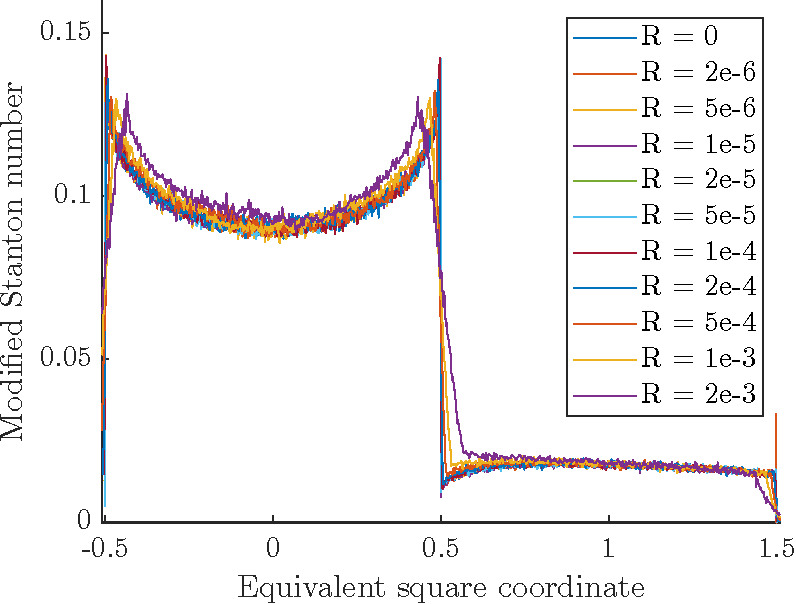
\includegraphics[width=0.52\textwidth]{Images/4. Results/Radius/stsec.pdf}
    \caption{Distribution of Stanton number along the square contour for varying values edge radius.}
    \label{fig:radiusstsec}
\end{figure}

\autoref{fig:radiusstsec} shows the Stanton number distribution around the geometry for varying values of edge radius (again, for clarity reasons only the test cases with comparatively small edge radius have been included). The distributions follows closely the one included in \autoref{fig:squarestsec} for $Kn = 0.01$, and very little change is observed for the peak Stanton number values (corresponding to the 0.5 point on the equivalent square coordinate axis) for varying values of edge radius. 



Plotting the Stanton number ratio against the local Knudsen number at the square corner (as shown in \autoref{fig:radiusstkn}) reveals an interesting trend. In the initial section of the Knudsen number range, the Stanton number ratio monotonically increases. However, as the local Knudsen number goes above 1, the Stanton ratio becomes virtually independent of it. 

This effect can be explained as follows: in the first part of the Knudsen number range the coalescence effect explained above is significant: as the edge radius is decreased, and thus Knudsen number is increased, the two peaks at the square corners are still separating, and the stagnation point heating is reducing. the ratio between the Stanton numbers at the two locations is thus increasing. Beyond a certain radius threshold, the geometry becomes virtually indistinguishable from a perfect square, and the effect stops being relevant.

\begin{figure}
    \centering
    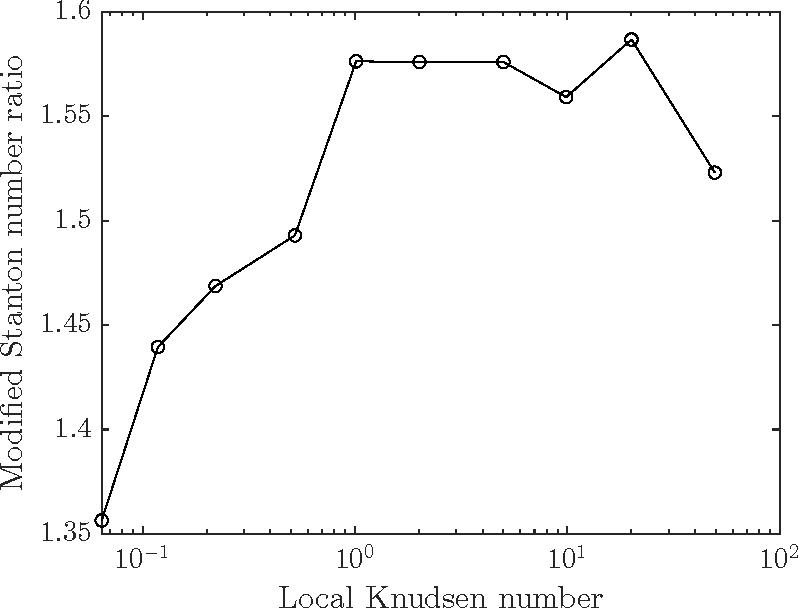
\includegraphics[width=0.52\textwidth]{Images/4. Results/Radius/stkn.pdf}
    \caption[Stanton number ratio vs local Knudsen number for the varying edge radius test case.]{Stanton number ratio vs local Knudsen number for the varying edge radius test case. Note that the datapoints included are the ones from the test cases in \autoref{fig:radiusstsec}.}
    \label{fig:radiusstkn}
\end{figure}

The second section of the graph also gives some relevant insight: as the Stanton ratio does not increase or decrease with local Knudsen number, the change observed in \autoref{fig:ratiokn} could be only due to a change in global Knudsen number.

\subsection{Constant local Knudsen number results}
\autoref{fig:localhtsec} and \autoref{fig:localstsec} respectively show the heat transfer and Stanton number distribution along the square contour for the constant local Knudsen number case. As shown in \autoref{tab:local}, a radius reduction corresponded to an equivalent Knudsen number increase, with the aim of maintaining the local Knudsen number constant. This objective was unfortunately not reached, as the theorised proportionality between local and global Knudsen numbers proved to not be valid.

Features noted when independently varying global Knudsen number and edge radius are both present, such as the more gentle decrease in heat transfer past the square corner or the order of magnitude increase in heat transfer. From \autoref{fig:localstsec} it is possible to note the presence of a Stanton number peak at the corner of the $Kn = 10$ case. Computing the local Knudsen number (equal to approximately \num{2e5}) reveals that this peak is probably caused by a very significant local rarefaction zone.

\autoref{fig:localstkn} shows the variation in Stanton number with local Knudsen number for the constant local Knudsen number case. The trend looks very similar to the one observed in \autoref{fig:ratiokn}.

\begin{figure}[H]
    \centering
    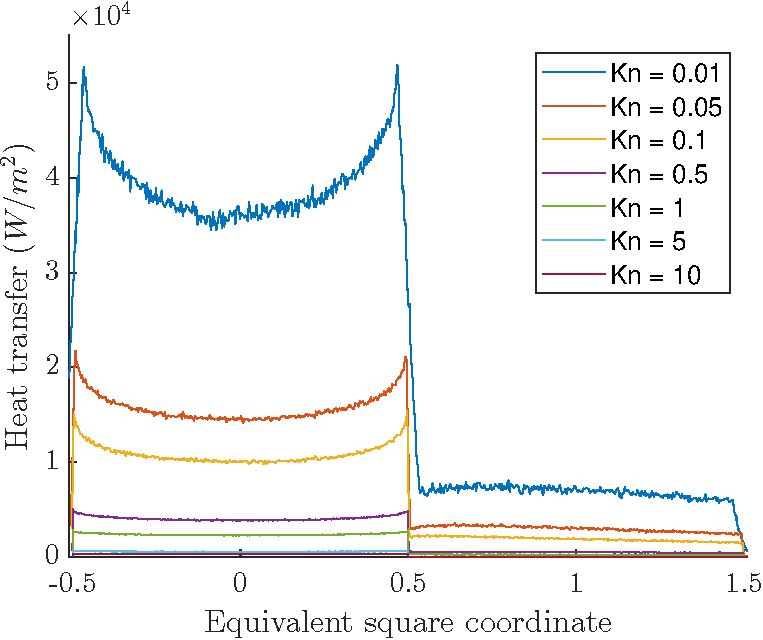
\includegraphics[width=0.52\textwidth]{Images/4. Results/local/htsec.pdf}
    \caption{Distribution of heat transfer along the square contour for constant local Knudsen number case.}
    \label{fig:localhtsec}
\end{figure}

\begin{figure}[H]
    \centering
    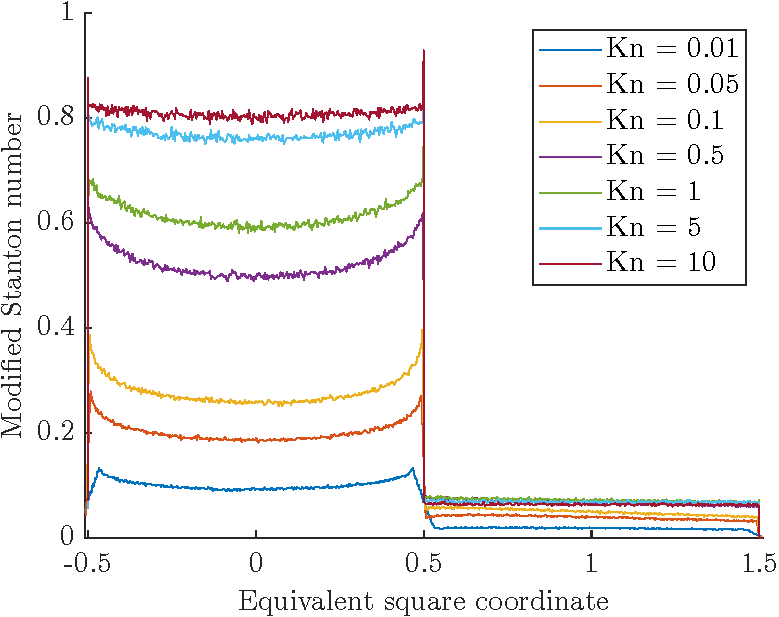
\includegraphics[width=0.52\textwidth]{Images/4. Results/local/stsec.pdf}
    \caption{Distribution of Stanton number along the square contour for constant local Knudsen number case.}
    \label{fig:localstsec}
\end{figure}

\begin{figure}[H]
    \centering
    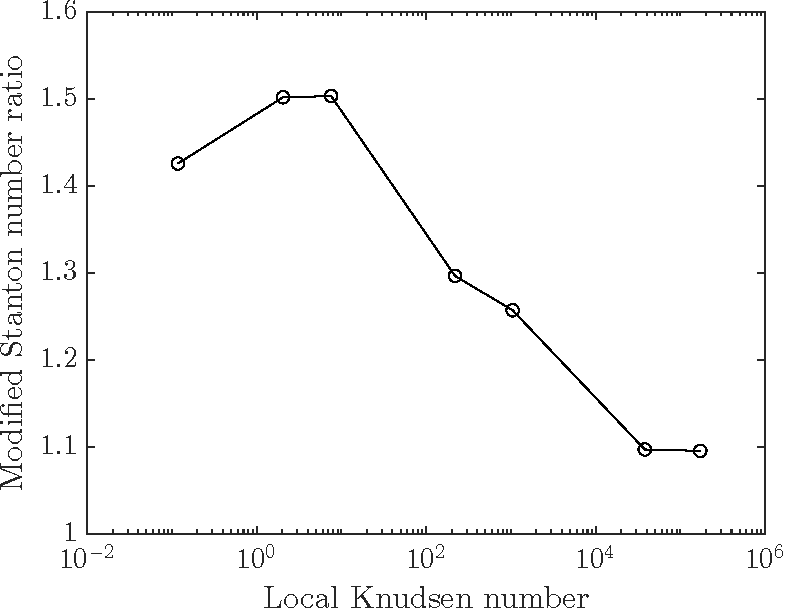
\includegraphics[width=0.52\textwidth]{Images/4. Results/local/stkn.pdf}
    \caption{Stanton number ratio vs local Knudsen number for constant local Knudsen number case.}
    \label{fig:localstkn}
\end{figure}

\subsection{Variation of angle of attack results}

\autoref{fig:aoa} shows the distribution of heat transfer along the square contour for varying values of angle of attack. As it is possible to see from it, the increase in heat transfer seen in literature \cite{pallahrini, spartavalid} has also been observed here.


\begin{figure}[H]
    \centering
    \begin{subfigure}{0.49\textwidth}
        \centering
        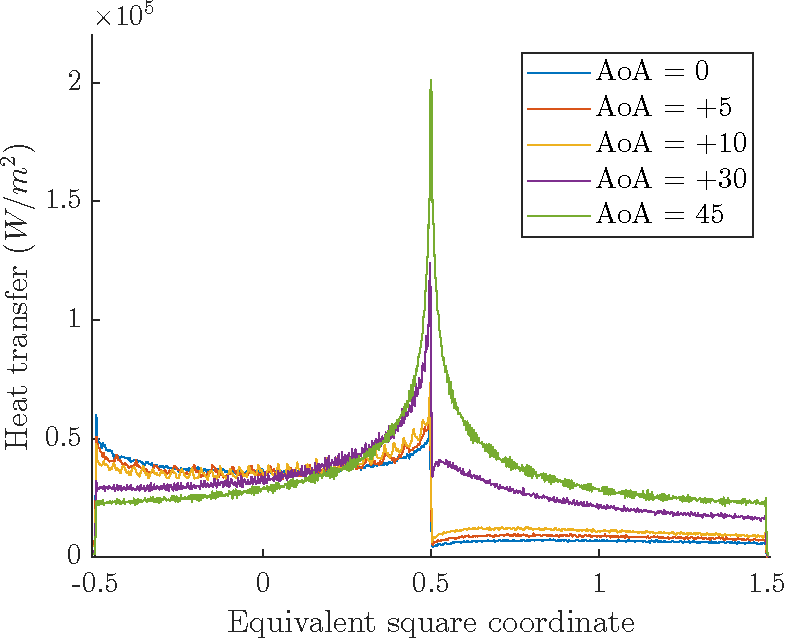
\includegraphics[width=\textwidth]{Images/4. Results/AoA/stsec+.pdf}
    \end{subfigure}
    \hfill
    \begin{subfigure}{0.49\textwidth}
        \centering
        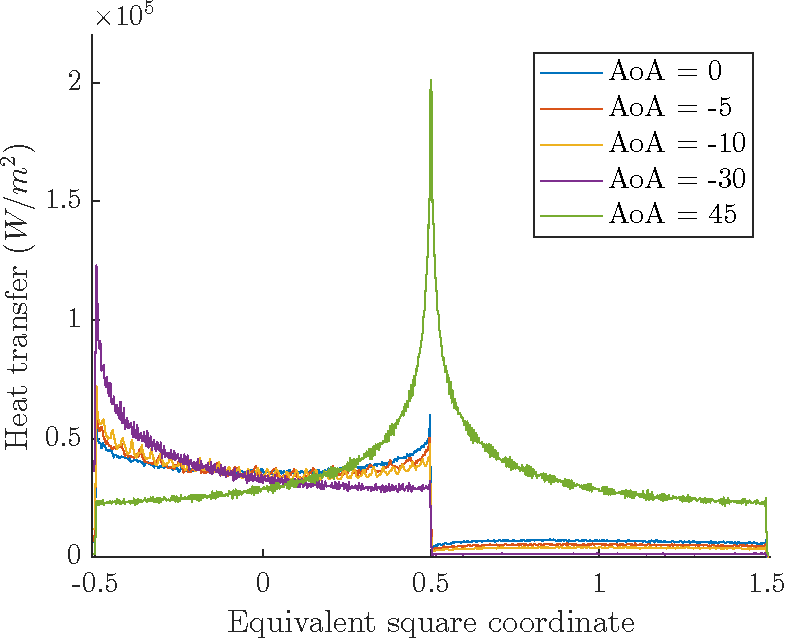
\includegraphics[width=\textwidth]{Images/4. Results/AoA/stsec-.pdf}
    \end{subfigure}
    \caption{Distribution of heat transfer along the square contour for varying values of angle of attack.}
    \label{fig:aoa}
\end{figure}

\subsection{Comparison of Stanton number ratio results}
\label{subsection:comparison}
The results obtained for the Stanton number variation with Knudsen number from the three test cases appear to be almost contradictory. The varying Knudsen number simulations show an explicit dependence on Knudsen number. This, coupled with the results of the varying radius simulations, which show an explicit independence of Stanton number with corner radius, would lead to believe that the change in Stanton number is only due to a change in density. However, if this was the case, the constant local Knudsen number simulation would have to only be dependent on global Knudsen number, and thus replicate the section of \autoref{fig:ratiokn} between the $Kn = 1$ and $Kn = 100$ (as the global Knudsen numbers of these datapoints match the ones used for the constant local Knudsen number simulations.

The decrease in ratio observed in \autoref{fig:ratiokn} and \autoref{fig:localstkn} is also of unknown origin. If it had been only observed in the varying Knudsen number case it could have probably been attributed to an unconverged mesh, as grid independence was not proven for a global Knudsen number of 0.001. However, the fact that this decrease has also been seen in the constant local Knudsen number case invalidates this theory, since the global Knudsen number for the first datapoint was equal to 0.01 (which was validated by mesh convergence)

Overall, this phenomenon appears to be quite complex, and further research is needed to identify a satisfactory correction factor to be implemented in rapid prototyping codes. This further research could be directed into modelling the lower Knudsen number regions through pure CFD or coupled DSMC-CFD codes, in order to provide some useful insight for the development of a valid correction factor.

\subsection{General considerations on the Direct Simulation Monte Carlo technique}
\label{subsection:dsmcdisc}
Direct Simulation Monte Carlo has overall proven to be a very useful and precise tool for the analysis of rarefied flows. Its computational cost prevents it however from leaving the academic setting, as powerful computing clusters are required for accurately simulating even very small domains: in the work carried out for this research thesis most of the simulations were run over multiple days on 40 state of the art server computing cores, despite the domain being limited to a 30 by \qty{30}{\cm} 2D square.
Employing this tool for full 3D simulations, larger domains or the modelling of the pure continuum regime remains thus still unfeasible, if not through the use of coupled DSMC-CFD codes or very powerful supercomputers.
\newpage

\section{Conclusion and future work}
The objective of this research was to analyse the effect of local and global rarefaction zones on the heat transfer onto simple shapes. 

In \autoref{1} a significant increase in the interest in space exploration was highlighted, and the need for new aerodynamic decelerators was evidenced. Moreover, it was pointed out that research into hypersonic rarefied flows is needed to develop the aforementioned aeroshells. 

In \autoref{section:2} the theoretical background for rarefied flow was outlined, and relevant research in the field examined. It was discovered that the optimal way to model this flow regime is through Direct Simulation Monte Carlo.

In \autoref{section:3} the working principles of DSMC were outlined, and four set of simulations on simple shapes (varying global Knudsen number, varying edge radius, constant local Knudsen number and varying angle of attack) were designed based on them. Convergence studies were thus conducted and the simulation results were validated, in order to ensure the accuracy of the simulations.

In \autoref{section:4} the main findings were presented: 
\begin{itemize}
    \item A drastic change in flow physics with rarefaction was noted, and a theoretical explanation was provided.
    \item The dependence of stagnation point Stanton number on global Knudsen number was evidenced and verified through comparison with literature.
    \item The dependence of the ratio between peak and stagnation point Stanton number with Knudsen number was investigated, in order to determine a correction factor for aerothermodynamic rapid prototyping codes. It was however discovered that further research is required, directed especially towards the continuum flow regime.
\end{itemize}

Overall, the research conducted can be considered successful regarding the investigation into the effects of rarefaction. More work is however needed to obtain a valid correction factor.
\clearpage

{\small
\bibliographystyle{unsrtnat}
\bibliography{export}
}

\end{document}
